\documentclass[8pt]{beamer}
\usepackage[nobglogo]{beamerthemedmi-owled}
\usepackage[utf8x]{inputenc}
\usepackage{default}
\usepackage{url}
\usepackage{verbatim}
\usepackage{graphicx}
\usepackage{mathrsfs}
\usepackage{dl}
\usepackage{mls}
%\usepackage{listings}


\mode<presentation>
{
  \usetheme{dmi-owled}
  %\usetheme{Warsaw}
  % or ...

  \setbeamercovered{transparent}
  % or whatever (possibly just delete it)
}

\title{Linked Open Data e Semantic Web:\\
Fondamenti e Linguaggi di Interrogazione\\
Parte Prima}

\author{Cristiano Longo\\ 
{\small{longo@dmi.unict.it}}}



\date{Universit\`a di Catania, 11/11/2016}
\newcommand{\urlsingle}[1]{{\small {\center {\url{#1}}}}}
\begin{document}
\maketitle
\setcounter{tocdepth}{1}

\section{Introduzione}

\section{Open Data}
\begin{frame}
	\frametitle{Open Knowledge}
	\begin{quote}
SEE HOW DATA CAN CHANGE THE WORLD

A world where knowledge creates power for the many, not the few.

A world where data frees us — to make informed choices about how we live, what we buy and who gets our vote.

A world where information and insights are accessible — and apparent — to everyone.

This is the world we choose.	
	\end{quote}
	
	da Open Knowledge Foundation.\footnote{https://okfn.org/}
\end{frame}

\begin{frame}
\frametitle{The Open Definition}

\begin{quote}
Open means anyone can freely access, use, modify, and share for any purpose (subject, at most, to requirements that preserve provenance and openness).\footnote{\url{http://opendefinition.org}} 
\end{quote}
\end{frame}

\begin{frame}
\frametitle{Formati Aperti}

Dalle \emph{LINEE GUIDA NAZIONALI PER LA VALORIZZAZIONE DEL PATRIMONIO
INFORMATIVO PUBBLICO}:
\vspace{\baselineskip}

a) \emph{formati aperto}, un formato di dati reso pubblico, documentato
esaustivamente e neutro rispetto agli strumenti tecnologici necessari per la fruizione dei dati stessi (esempi sono
XML, JSON, ODF, \ldots);

\end{frame}

\begin{frame}
\frametitle{Dati Aperti}

Dalle \emph{LINEE GUIDA NAZIONALI PER LA VALORIZZAZIONE DEL PATRIMONIO
INFORMATIVO PUBBLICO}:
\vspace{\baselineskip}

b) \emph{dati di tipo aperto}, i dati che presentano le seguenti caratteristiche:
\vspace{\baselineskip}

1) sono disponibili secondo i termini di una \emph{licenza} che ne permetta
l'utilizzo da parte di chiunque, anche per finalit\`a commerciali, in formato
disaggregato (esempi di licenze sono Creative Commons e Apache License);
\vspace{\baselineskip}

\uncover<2->{
2) sono \emph{accessibili} attraverso le tecnologie dell'informazione e della
comunicazione [\ldots] }
\vspace{\baselineskip}

\uncover<3->{
in \emph{formati aperti},
}
\vspace{\baselineskip}

\uncover<4->{
sono adatti all'utilizzo
automatico da parte di programmi per elaboratori 
}
\vspace{\baselineskip}

\uncover<5->{
e sono provvisti dei relativi \emph{metadati};
\vspace{\baselineskip}
}

\uncover<6->{
3) sono resi disponibili \emph{gratuitamente} [\ldots] oppure sono resi
disponibili ai costi marginali sostenuti per la loro riproduzione e divulgazione. 
}
\end{frame}

\begin{frame}
\frametitle{Dati Aperti della PA}
L'apertura dei dati in possesso della Pubblica Amminstrazione riveste
particolare importanze. Alcune ricadute dell'apertura di questi dati:
\vspace{\baselineskip}

\begin{itemize} [<+->]
 \item Economici
 \begin{itemize}
  \item redazione di business plan (vedi l'articolo sui flussi turistici\footnote{\url{http://opendatasicilia.it/2015/05/13/flussi-turistici-e-fruizione-dei-beni-culturali-catania-dal-2012-al-2013/}}),
  \item creazione di nuove imprese basate sui dati (vedi ad esempio \emph{Open Data 500}\footnote{\url{http://www.opendata500.com/us/list/}});
 \end{itemize}
 \item realizzazione di nuovi servizi per i cittadini (vedi ad esempio PETRUSINO,\footnote{\url{http://petrusino.opendatasicilia.it/}}
 ConfiscatiBene,\footnote{\url{http://www.confiscatibene.it/it}} Ordnance Survey,\footnote{\url{https://www.ordnancesurvey.co.uk/innovate/showcase}} Europeana);\footnote{\url{http://labs.europeana.eu/apps}}
 \item trasparenza (vedi ad esempio \url{soldipubblici.it} oppure \url{http://parlamento17.openpolis.it/});
 \item governo partecipato (uno strumento ad esempio è \url{http://www.normattiva.it/}).
\end{itemize}
\end{frame}

\begin{frame}
\frametitle{Dati Aperti della PA - Esempi}
Alcune esempi di pubbliche amministrazioni che hanno pubblicato i dati:
\vspace{\baselineskip}

\begin{itemize}
 \item Centrali
 \begin{itemize}
  \item Camera (\url{http://dati.camera.it/}) e Senato (\url{http://dati.senato.it/}) della Repubblica Italiana,
  \item ISTAT (\url{http://dati.istat.it/}),  
  \item Ministero per i Beni e le Attivit\`a Culturali e Turismo (\url{http://www.beniculturali.it/mibac/export/MiBAC/sito-MiBAC/MenuPrincipale/Trasparenza/Open-Data/index.html}, \url{http://www.beniculturali.it/mibac/opencms/MiBAC/sito-MiBAC/MenuPrincipale/LuoghiDellaCultura/Ricerca/index.html});  
 \end{itemize}
 \item Regioni
 \begin{itemize}
  \item Emilia Romagna (\url{http://dati.emilia-romagna.it}),
  \item Lombardia (\url{https://www.dati.lombardia.it}), 
  \item Piemonte (\url{http://www.dati.piemonte.it}), 
  \item Puglia (\url{www.dati.puglia.it}),
  \item Toscana (\url{http://dati.toscana.it}), 
  \item Umbria (\url{http://dati.umbria.it});
 \end{itemize}
 \item Provincie - Provincia Autonoma di Trento e Bolzano (\url{http://dati.trentino.it});
 \item Comuni
 \begin{itemize}
  \item Catania (\url{http://opendata.comune.catania.gov.it}),
  \item Palermo (\url{http://www.comune.palermo.it/opendata_menus.php}),
  \item Matera (\url{http://dati.comune.matera.it}).
 \end{itemize}
\end{itemize}
\end{frame}

\begin{frame}
	\frametitle{Dati Aperti della PA - Tipologie}
	Riportiamo a titolo esemplificativo l'elenco di categorie dei dataset presenti
	su \url{http://dati.emilia-romagna.it/} : 
	\begin{itemize}
	  \item Agricoltura
	  \item Ambiente
	  \item Bilancio
	  \item Bilancio Consuntivo
	  \item Bilancio di Previsione
	  \item Cartografia
	  \item Dati di Bilancio
	  \item Edilizia
	  \item Geologia
	  \item Geomorfologia
	  \item Mobilit\`a 
	  \item Pianificazione agricola
	  \item Processi Geologici 
	  \item Suolo 
	  \item Territorio
	  \item Turismo  
	  \item amministrazione  
	  \item istruzione 
	  \item popolazione
	\end{itemize}
\end{frame}
\begin{frame}
\frametitle{World Wide Web Consortium}
Il \emph{World Wide Web Consortium} (in breve \emph{W3C}, vedi \url{http://www.w3.org}) 
\`e un consorzio di standardizzazione per il Web che
conta 403 membri tra aziende e organizzazioni governative: CNR,
Microsoft Corporation, Apple Inc., Intel Corporation, Facebook, Google Inc., \ldots
\vspace{\baselineskip}

Altri standard sviluppati in seno al W3C sono: URL, HTTP, XML, HTML, CSS, SOAP, 
WSDL, Javascript. 
\end{frame}

\begin{frame}
  \frametitle{Classificazione 5 Stelle}

  Il w3c propone un modello per la qualit\`a degli open data denominato
  \emph{classificazione a 5 stelle}.\footnote{\url{http://5stardata.info}}
  \vspace{\baselineskip}  
  
  \begin{figure}
     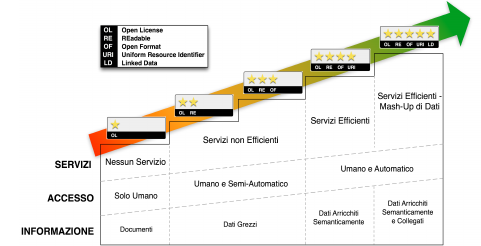
\includegraphics[width=300px]{5stelle_classificazione.png} 
    %\caption{Modello di classificazione per i metadati.\footnote{Dalle \emph{Linee guida nazionali per il patrimonio informativo pubblico (2014)}.}  
  \end{figure}
\end{frame}

\begin{frame}
  \frametitle{Classificazione 5 Stelle - Dimensioni}
  La classificazione 5 stelle viene estesa dall'AgID con alcune \emph{dimensioni}
  esplicative:
  \begin{itemize}[<+->]
   \item \emph{INFORMAZIONE} - descrive la qualit\`a dell'informazione fornita insieme ai dati;
   \item \emph{ACCESSO} -  descrive la facilit\`a con cui utenti e programmi riescono ad accedere ai dati;
   \item \emph{SERVIZI} - riguarda le tipologie e l'\emph{efficienza} dei servizi che possono essere realizzati a partire 
   dai dati.
  \end{itemize}
\end{frame}

  
\begin{frame}
  \frametitle{Classificazione 5 Stelle - Una Stella}
  
  Una Stella: Open Licence
  
  \begin{figure}
     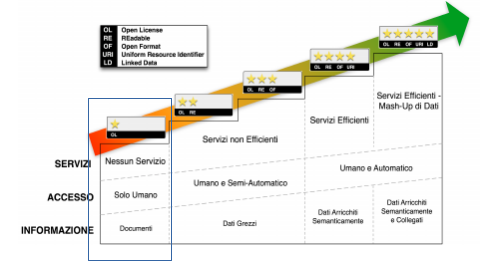
\includegraphics[width=180px]{stella1.png} 
    %\caption{Modello di classificazione per i metadati.\footnote{Dalle \emph{Linee guida nazionali per il patrimonio informativo pubblico (2014)}.}  
  \end{figure}
  
  La \emph{prima stella} si ottiene rilasciando i dati in qualunque formato
  ma con una \emph{licenza aperta}.
  Rientrano in questa categoria ad esempio le scansioni dei documenti.
  \vspace{\baselineskip}

  \begin{itemize}[<+->]
   \item \emph{INFORMAZIONE: documenti} - i dati sono incorporati all’interno di documenti senza struttura;
   \item \emph{ACCESSO: solo umano} - solo gli umani sono in grado di leggere i documenti senza struttura 
   e quindi dare un senso ai dati in esso presenti;
   \item \emph{SERVIZI: nessuno} può essere abilitato a meno di significativi interventi umani 
   di estrazione ed elaborazione;
  \end{itemize}
\end{frame}

\begin{frame}
  \frametitle{Classificazione 5 Stelle - Due Stelle}
  
    Due Stelle: Open Licence, (Machine) Readable

  \begin{figure}
     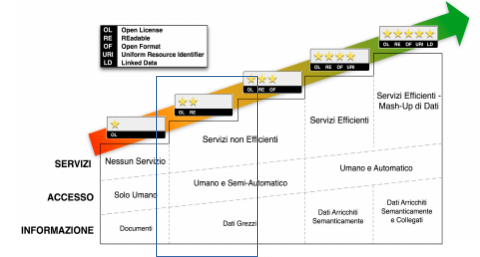
\includegraphics[width=180px]{stella2.png} 
    %\caption{Modello di classificazione per i metadati.\footnote{Dalle \emph{Linee guida nazionali per il patrimonio informativo pubblico (2014)}.}  
  \end{figure}
  
  La \emph{seconda stella} si ottiene se i dati sono forniti in un formato leggibile 
  da un agente automatico. 
  
  Rientrano in questa categoria ad esempio i files in formato \emph{excel}.
  \vspace{\baselineskip}

  \begin{itemize}[<+->]
   \item \emph{INFORMAZIONE: dati grezzi (o semi-strutturati)} - i dati sono leggibili anche da un programma 
   ma necessita un intervento umano per interpretarli;
   \item \emph{ACCESSO: umano e semi-automatico} - i software possono leggere i dati ma non sono in grado di
   interpretarli automaticamente;
   \item \emph{SERVIZI: non efficienti} - servizi realizzati ad-hoc e devono incorporare al loro
  interno i dati;
  \end{itemize}
\end{frame}

\begin{frame}
  \frametitle{Classificazione 5 Stelle - Tre Stelle}
  
  Tre Stelle: Open Licence, (Machine) Readable, Open Format

  \begin{figure}
     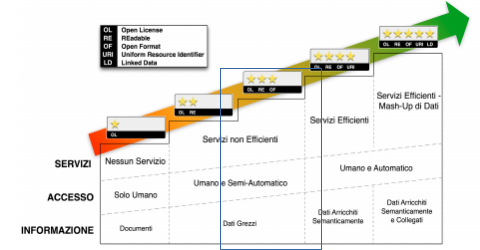
\includegraphics[width=180px]{stella3.png} 
    %\caption{Modello di classificazione per i metadati.\footnote{Dalle \emph{Linee guida nazionali per il patrimonio informativo pubblico (2014)}.}  
  \end{figure}
  
  La \emph{terza stella} viene attribuita se i dati sono rilasciati in un formato \emph{aperto}.
  Rientrano in questa categoria ad esempio i files \emph{jsono}, \emph{csv}, \emph{xml}.
  \vspace{\baselineskip}

  \begin{itemize}
   \item \emph{INFORMAZIONE: dati grezzi (o semi-strutturati)} - i dati sono leggibili anche da un programma 
   ma necessita un intervento umano per interpretarli;
   \item \emph{ACCESSO: umano e semi-automatico} - i software possono leggere i dati ma non sono in grado di
   interpretarli automaticamente;
   \item \emph{SERVIZI: non efficienti} - servizi realizzati ad-hoc e devono incorporare al loro
  interno i dati;
  \end{itemize}
\end{frame}

\begin{frame}
  \frametitle{Classificazione 5 Stelle - Quattro Stelle}
  
  Quattro Stelle: Open Licence, (Machine) Readable, Open Format, URI

  \begin{figure}
     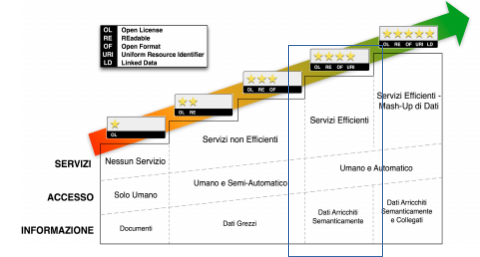
\includegraphics[width=180px]{stella4.png} 
    %\caption{Modello di classificazione per i metadati.\footnote{Dalle \emph{Linee guida nazionali per il patrimonio informativo pubblico (2014)}.}  
  \end{figure}
  
  La \emph{quarta stella} si ottiene esponendo i dati con le tecnologie del web semantico (RDF e SPARQL).
  \vspace{\baselineskip}

  \begin{itemize}[<+->]
   \item \emph{INFORMAZIONE: dati arricchiti semanticamente} - i dati sono descritti usando tecnologie del Web Semantico;
   \item \emph{ACCESSO: umano e automatico} - i software sono in grado di elaborare i dati quasi senza ulteriori 
   interventi umani (livelli 4 e 5);
   \item \emph{SERVIZI: efficienti} - servizi che sfruttano accessi diretti a Web per reperire i dati.
  \end{itemize}
\end{frame}

\begin{frame}
  \frametitle{Classificazione 5 Stelle - Cinque Stelle}
  
  Cinque Stelle: Open Licence, (Machine) Readable, Open Format, URI, \emph{Linked} Data

  \begin{figure}
     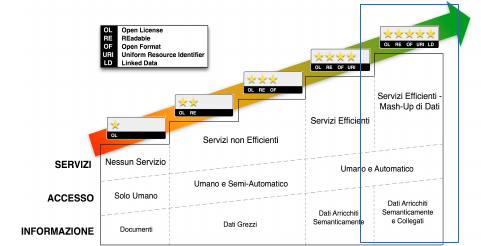
\includegraphics[width=180px]{stella5.png} 
    %\caption{Modello di classificazione per i metadati.\footnote{Dalle \emph{Linee guida nazionali per il patrimonio informativo pubblico (2014)}.}  
  \end{figure}
  
  La \emph{quinta stella} viene attribuita quando i dati contengono riferimenti a dataset di terze parti.
  \vspace{\baselineskip}

  \begin{itemize}[<+->]
   \item \emph{INFORMAZIONE: dati arricchiti semanticamente} - i dati sono descritti usando tecnologie del Web Semantico;
   \item \emph{ACCESSO: umano e automatico} - i software sono in grado di elaborare i dati quasi senza ulteriori 
   interventi umani (livelli 4 e 5);
   \item \emph{SERVIZI: efficienti e con mashup di dati} - servizi che sfruttano sia accessi diretti a Web 
   sia l'informazione ulteriore catturata attraverso i \emph{link} dei dati di interesse.
  \end{itemize}
\end{frame}

\begin{frame}
  \frametitle{Classificazione 5 Stelle - Cinque Stelle - Esempio}
  
  Cinque Stelle: Open Licence, (Machine) Readable, Open Format, URI, \emph{Linked} Data
  \vspace{\baselineskip}
  
  In altre parole, \`e possibile collegare dataset differenti ed eterogenei.
  Nell'esempio che segue i diversi colori indicano le collocazioni degli
  elementi e delle informazioni in dataset differenti.

  \begin{figure}
     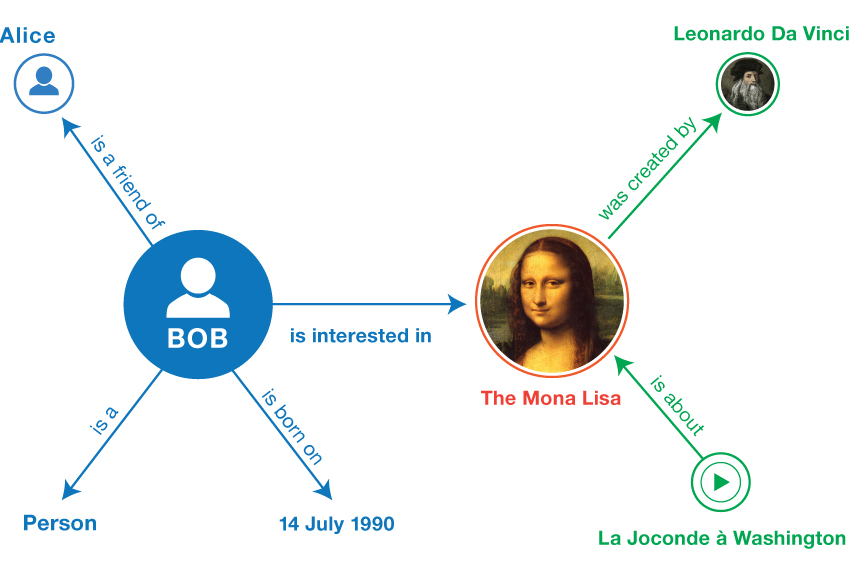
\includegraphics[width=220px]{example-graph.jpg} 
  \end{figure}  
\end{frame}

\section{Semantic Web}
\begin{frame}
\frametitle{World Wide Web - nascita}
\begin{quote}
Imagine, then, the references in this document all being associated with 
the network address of the thing to which they referred, so that while 
reading this document you could skip to them with a click of the mouse.
\end{quote}
\vspace{\baselineskip}
\emph{Semantic Web Roadmap}, Tim Berners-Lee, 1989.
\vspace{\baselineskip}

\uncover<2->{
Nel 1993 il CERN rilascer\`a di pubblico dominio i primi software per il
world wide web, tra cui il primo browser chiamato per l'appunto \emph{World
Wide Web}.\footnote{\url{http://home.cern/topics/birth-web}} 
}
\end{frame}

\begin{frame}
\frametitle{World Wide Web - definizione}
\begin{quote}
The World Wide Web (WWW, or simply Web) is an information space in which
the items of interest, referred to as resources, are identified by global
identifiers called Uniform Resource Identifiers (URI).
\end{quote}
\vspace{\baselineskip}
\emph{Architecture of the World Wide Web, Volume
I}\footnote{\url{https://www.w3.org/TR/webarch/}}
\vspace{\baselineskip}

\uncover<2->{
Le prime specifiche rilasciate furono:
\begin{itemize}
  \item Uniform Resource Locators (URLs),
  \item Hypertext Transfer Protocol (HTTP),
  \item Hypertext Markup Language (HTML).
\end{itemize}
}
\end{frame}

\begin{frame}
\frametitle{Limiti del World Wide Web (1/4)}
\begin{quote}
The Web was designed as an information space, with the goal that it should be 
useful not only for human-human communication, but also that machines would be
able to participate and help. One of the major obstacles to this has been the
fact \textbf{that most information on the Web is designed for human consumption}, and 
even if it was derived from a database with well defined meanings (in at least 
some terms) for its columns, that \textbf{the structure of the data is not evident to 
a robot browsing the web.}  
\end{quote}
\vspace{\baselineskip}
\emph{Semantic Web Roadmap}, Tim Berners-Lee, 1998.
\end{frame}

\begin{frame}
\frametitle{Limiti del World Wide Web (2/4)}
Alcuni problemi nell'interpretazione di testi derivano da:
\begin{description}
 \item[Lingue Differenti] e.g. $Parigi$ e $Paris$ possono indicare la stessa citt\`a.
 \item[Omonimie] e.g. esistono svariate citt\`a chiamate 
 \emph{Paris} nel mondo (Arkansas, Idaho, Illinois, Kentucky,
 Maine, Michigan, Missouri, New York, \ldots);
\end{description}
\end{frame}

\begin{frame}
\frametitle{Limiti del World Wide Web (3/4)}

La situazione si complica in presenza di contenuti multimediali.

\begin{figure}
    
\includegraphics[width=250px]{unrecognizable.jpg} 
\end{figure}
\end{frame}

\begin{frame}
\frametitle{Limiti del World Wide Web (4/4)}
Come conseguenza, spesso \`e impossibile eseguire su web ricerce 
\emph{complesse} ottenendo risultati accurati. Ad esempio, cercando sul web
\emph{``Federico II places''} non si ottengono risultati in prima pagina su 
Federico II, ma solo sull'omonima universit\`a:
  
  \begin{small}
    \begin{enumerate}
   \item Universit\`a degli Studi di Napoli "Federico II" | OPEN Places
   \item AOU - Policlinico "Federico II" - Napoli, Italy - Hospital | Facebook
   \item Federico II Ingegneria Via Claudio - College and University | Facebook
   \item MARIA CATERINA FONTE - www.docenti.unina.it
  \end{enumerate}
  \end{small}
\end{frame}

\begin{frame}
\frametitle{Il Web Semantico (1/2)}
\begin{quote}
[\ldots] the Semantic Web approach instead develops languages for expressing
information in a machine processable form. 
\end{quote}
\emph{Semantic Web Roadmap}, Tim Berners-Lee, 1998.

\begin{figure}
    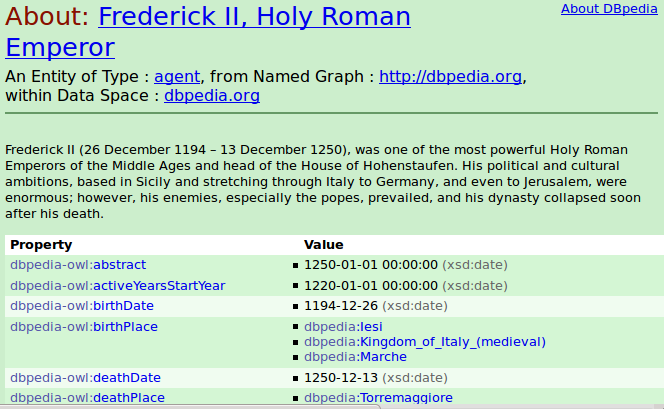
\includegraphics[width=250px]{federicoII_dbpedia.png} 
    \caption{Federico II su dbpedia.org}
\end{figure}
\end{frame}

\begin{frame}
\frametitle{Il Web Semantico (2/2)}

 Il \emph{Web Semantico} nasce per associare informazioni 
 \emph{strutturate} alle pagine web, che solitamente sono
 composte da testo libero.\footnote{Vedi \emph{Semantic Web Roadmap}, Tim Berners-Lee, 1998.}
 \vspace{\baselineskip}

\uncover<2->{
I \emph{linguaggi di rappresentazione} usati nel Web semantico 
hanno una \emph{sintassi rigorosa} e sono dotati di una \emph{semantica formale}.
\vspace{\baselineskip}
}

\uncover<3->{
Questo rende possibile effettuare interrogazioni complesse sui dataset, 
ottenendo dei risultati precisi anche se a volte parziali:

\begin{center}
Q = “Luoghi di nascita di Federico II e dei suoi parenti stretti” . 
\end{center}
}
\end{frame}

\begin{frame}
\frametitle{Il Web Semantico - Vocabolari}

 L'utilizzo di \emph{vocabolari} condivisi e universalmente riconisciuti,
 spesso dedicati a specifici domini di conoscenza, garantisce
 l'interoperabilit\`a applicativa.
 
\uncover<2->{
 Un esempio di vocabolario \`e \emph{ISA Programme Location Core Vocabulary
 (LOCN).}\footnote{\url{https://www.w3.org/ns/locn}} 
 
 \begin{quote}
 The ISA Programme Location Core Vocabulary provides a minimum set of classes
 and properties for describing any place in terms of its name, address or geometry.
 \end{quote}
}

\uncover<3->{
 \`E possibile realizzare applicativi in grado di trattare informazioni espresse
 con questo vocabolario senza tener conto di chi pubblica le informazioni e
 come.
}
\end{frame}

\begin{frame}
\frametitle{Il Web Semantico - Semantica}

I \emph{linguaggi di rappresentazione} usati nel Web semantico 
sono dotati di una \emph{semantica formale} mutuata dai 
\emph{sistemi di rappresentazione della conoscenza}\footnote{Vedi
Brachman, Schmolze (1985) \emph{An Overview of the KL-ONE Knowledge
Representation System}} e dalle \emph{logiche descrittive}.\footnote{Vedi 
Baader, Calvanese, McGuinness, Nardi, Patel-Schneider \emph{The Description 
Logic Handbook: Theory, Implementation, and Applications, 2nd Edition}.}
\vspace{\baselineskip}

\uncover<2->{
Questo permette di effettuare attivit\`a di \emph{reasoning} (in genere,
inferenze) per
estrarre \emph{conoscenza implicita}.
\vspace{\baselineskip}

Ad esempio, se \`e noto che ``Tutti gli esseri umani sono mortali''
un reasoning engine potr\`a dedurre che ``Socrate \`e mortale''
dal fatto che ``Socrate \`e umano''.
}
\end{frame}

\begin{frame}
\frametitle{Linked Data (1/2)}

I dataset nel Web Semantico possono essere \emph{collegati} tra loro. Ad esempio, una stessa risorsa pu\`o essere descritta 
sotto diversi aspetti in dataset differenti.
\vspace{\baselineskip}

Ad esempio, la citt\`a di Catania \`e presente:
\begin{itemize}
 \item come pubblica amministrazione nel dataset del sistema pubblico di connettivit\`a e cooperazione\footnote{\url{http://spcdata.digitpa.gov.it/}}
 con la url \url{http://spcdata.digitpa.gov.it/Amministrazione/c_c351};
 \item come divisione amministrativa nel dataset \url{http://www.geonames.org};
 \item come area territoriale nel dataset dell'ISTAT  \url{http://linkedstat.spaziodati.eu/}.
\end{itemize}
\end{frame}

\begin{frame}
\frametitle{Linked Data (2/2)}
\`E possibile effettuare interrogazioni che coinvolgano diversi
dataset (anche eterogenei).
\vspace{\baselineskip}

Ad esempio, la seguente query pu\`o essere eseguita
interrogando un data set contenente dati storici ed uno 
sulle strutture ricettive:


\begin{center}
Q = “Strutture ricettive nei luoghi di nascita di Federico II e dei suoi parenti stretti.”
\end{center}
\end{frame}

\begin{frame}
\frametitle{Linked Open Data Cloud (1/2)}
\begin{quote}
The Semantic Web is a web of data, in some ways like a global database.
\end{quote}
\small{\emph{Semantic Web Roadmap}, Tim Berners-Lee, 1998.}
\begin{figure}
    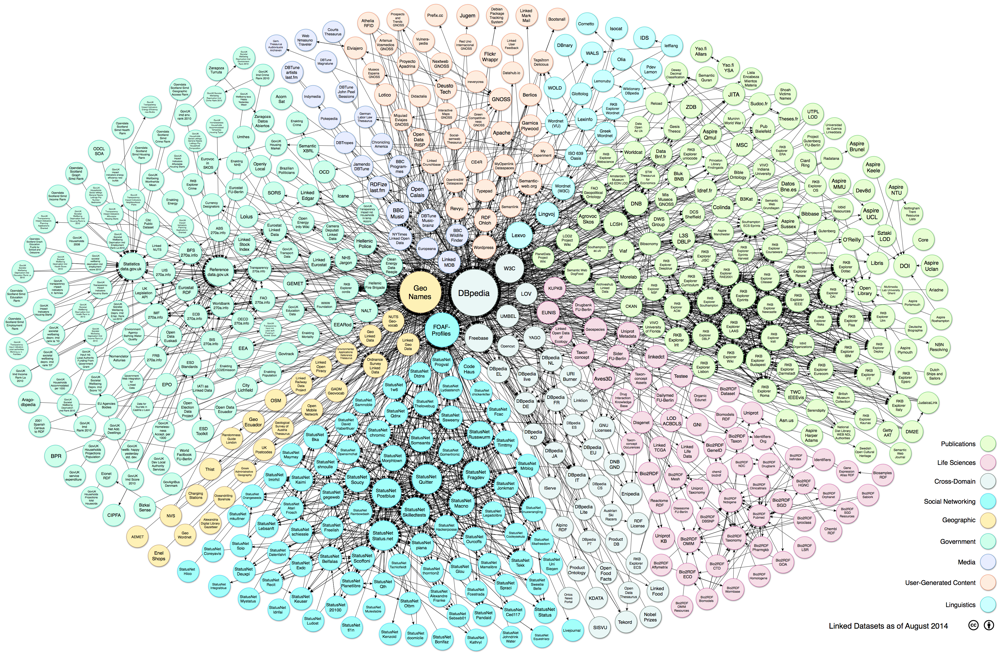
\includegraphics[width=250px]{lod-cloud_colored_1000px.png} 
    \caption{Linked Open Data Cloud}
\end{figure}
\end{frame}

\begin{frame}
\frametitle{Linked Open Data Cloud (2/2)}
Nel \emph{Linked Open Data Cloud} sono presenti 365 dataset (fonte \url{http://stats.lod2.eu/}).
\vspace{\baselineskip}

Alcuni dataset:
\begin{itemize}
 \item \emph{DBPedia} (\url{dbpedia.org}) corrispondente a \url{wikipedia.org};
 \item \emph{Linked Movie Database} (\url{http://linkedmdb.org/}) controparte sul Web Semantico di \emph{Internet Movie Database} 
 (\url{http://www.imdb.com/});
 \item \emph{Linked GeoData} (\url{http://linkedgeodata.org}) 
  contiene i dati di \emph{OpenStreetMap} (\url{http://www.openstreetmap.org/});
  \item \emph{AGROVOC} (\url{http://aims.fao.org/agrovoc}) \`e il dataset della FAO (\url{http://fao.org});
  \item \emph{Europeana} (\url{http://pro.europeana.eu/linked-open-data}) contiene dati su beni culturali e tradizioni Europee. 
\end{itemize}

\uncover<2->{
  \emph{LodLive}\footnote{\url{http://lodlive.it}}
  e \emph{LodView}\footnote{\url{http://lodview.it}} sono due servizi online
  che permettono di navigare il Linked Open Data Cloud ed esaminare le informazioni
  in esso contenute in merito ad uno specifico elemento.
}  
\end{frame}


\section{Ontologie}
\begin{frame}
\frametitle{Ontologie}
 I linguaggi di rappresentazione usati nel Web Semantico
 si basano tutti sulla nozione di \emph{ontologia}, mutuata
 dall'ambito dei sistemi di rappresentazione della conoscenza.
 \vspace{\baselineskip}
\vspace{\baselineskip}

Una \emph{ontologia} \`e una descrizione \emph{parziale} del mondo:
\begin{itemize}
 \item descrive una porzione del mondo, spesso \`e limitata ad un'unico \emph{dominio di conoscenza};
 \item non si assume che i fatti non esplicitamente presenti nell'ontologia siano falsi (\emph{Open World Assumption}).
\end{itemize}
\vspace{\baselineskip}

Essa \`e costituita da un insieme finito di \emph{affermazioni}. Ad esempio:
\begin{itemize}
 \item Tutti gli esseri umani sono mortali;
 \item Socrate \`e mortale;
 \item Alice \`e la madre di Roberto.
\end{itemize}
\end{frame}

\begin{frame}
\frametitle{Ontologie - Affermazioni}
Le affermazioni contenute in una ontologia sono di tre tipi:
\vspace{\baselineskip}

\emph{Constraints:} impongono dei vincoli \emph{semantici} sul dominio di conoscenza 
che si va a rappresentare. La notazione richiama quella insiemistica;
\vspace{\baselineskip}
\[
 HumanBeing \Issub Mortal 
\]
\emph{Property Assertions}: impongono una relazione tra due elementi del dominio;
\[
 Alice\,motherOf\,Bob 
\]
\emph{Class Assertions}: indicano l'appartenenza di un elemento ad un insieme.
\[
 HumanBeing(Socrate) 
\]
\end{frame}


\newcommand{\CNames}{N_C}
\newcommand{\PNames}{N_P}
\newcommand{\INames}{N_I}
\newcommand{\VNames}{V}

\begin{frame}
\frametitle{Ontologie - Sintassi}

Riportiamo la definizione formale per la sintassi delle ontologie.
\vspace{\baselineskip}

Siano $\CNames$, $\PNames$, $\INames$ tre insiemi infiniti, numerabili e 
a due a due disgiunti di nomi di \emph{classe}, \emph{propriet\`a} e \emph{individuo},
rispettivamente.
\vspace{\baselineskip}

Una \emph{ontologia} \`e un insieme finito di asserzioni dei seguenti tipi:
\[
 \begin{array}{ll}
  \mbox{(Constraints)} & C \Issub D\\
  & P \Issub Q \\
  & \dom(P) \Issub C \\
  & \range(P) \Issub C \\
  &\\
  \mbox{(Class Assertions)} & C(a)\\
  &\\
  \mbox{Property Assertions} & a\,P\,b\;(\mbox{equivalente }P(a,b))\\
 \end{array}
\]
dove $C, D \in \CNames$, $P, Q \in \PNames$ e $a, b \in \INames$.
\vspace{\baselineskip}

Si noti che la grammatica per i vincoli ivi riportata \`e \emph{minimale}.
Esistono linguaggi di rappresentazione che permettono di esprimere vincoli
pi\`u complessi.
\end{frame}

\newcommand{\Ont}{\mathcal{O}}
\newcommand{\Ontp}{\mathcal{O'}}

\begin{frame}
\frametitle{Ontologie - Esempio}
Riportiamo un esempio di ontologia. Siano $Human, Woman, Man, Male, Female \in
\CNames$, $relative, child \in \PNames$, $Alice, Bob, Charlie \in \INames$.
\vspace{\baselineskip}

\[
\begin{array}{ccl}
 \Ont = & \{ & Woman \Issub Human, \\
 &&Man \Issub Human, \\
 &&Woman \Issub Female, \\
 &&Man \Issub Male, \\
 &&Woman(Alice), \\
 &&Man(Bob),\\
 &&Alice\,relative\,Bob,\\ 
 &&Alice\,child\,Charlie \}
\end{array} 
\]
\end{frame}

\begin{frame}
\frametitle{Ontologie - L'Editor Prot\'eg\'e}

  \emph{Prot\'eg\'e}\footnote{\url{http://protege.stanford.edu/products.php}} 
  \`e una suite per la modellazione di ontologie del Web Semantico, disponibile 
  sia in versione web, che in versione installabile localmente (\emph{Prot\'eg\'e Desktop}).
  \vspace{\baselineskip}

\uncover<2->{
  Permette di definire gerarchie di classi (tab \emph{Classes}) a partire dalla
  classe radice \texttt{Thing}. Per ogni classe \`e possibile definire \emph{label} 
  e \emph{comment} come annotazioni.
  \vspace{\baselineskip}
}

\uncover<3->{
  Analogamente \`e possibile definire gerarchie di propriet\`a (tab \emph{Object Poperties}) 
  a partire dalla propriet\`a radice \texttt{topObjectProperty} e di definire annotazioni
  per le propriet\`a. Inoltre, \`e possibile imporre dei vincoli di dominio e codominio
  per le propriet\`a.
  \vspace{\baselineskip}
}

\uncover<4->{
  Infine \`e possibile definire degli individui (tab \emph{Individuals}) associarli 
  a delle classi di appartenenza e metterli in relazione tra loro attraverso delle
  propriet\`a.
  \vspace{\baselineskip}
}
\end{frame}

\begin{frame}
\frametitle{Ontologie - Interpretazioni}

Per definire la semantica delle ontologie \`e necessario prima introdurre
il concetto di interpretazione. 
\vspace{\baselineskip}

Una \emph{interpretazione} $\I=(\Delta^{\I}, \cdot^{\I})$ \`e una coppia
$\Delta^{\I}$, $\cdot^{\I}$ dove:
\begin{itemize}
 \item $\Delta^{\I}$ \`e un insieme non vuoto;
 \item $\cdot^{\I}$ \`e una funzione (polimorfa) che associa
 \begin{itemize}
  \item ad ogni nome di concetto in $\CNames$ un sottoinsieme di $\Delta^{\I}$,
  \item ad ogni nome di propriet\`a in $\PNames$ una relazione su $\Delta^{\I}$,
  \item ad ogni nome di individuo in $\INames$ un elemento di $\Delta^{\I}$.
 \end{itemize}
\end{itemize}
\vspace{\baselineskip}

\uncover<2->{
 Consideriamo ad esempio la seguente ontologia
 \begin{small}
\[
\begin{array}{ccc}
 \Ont = & \{ & Woman \Issub Human, Man \Issub Human, Woman \Issub Female, Man \Issub Male, \\
 &&Woman(Alice), Man(Bob), Alice\,relative\,Bob, Alice\,child\,Charlie \}
\end{array} 
\]
 \end{small}
 Una possibile interpretazione $\I$ \`e la seguente:
 \begin{small}
\[
 \begin{array}{lcl}
    \Delta^{\I} & = & \mathbb{N}\\
    Alice^{\I} & = & 0 \\
    Bob^{\I} & = & 1 \\
    Charlie^{\I} & = & 2 \\
    Human^{\I} & = & \{ 0, 1, 2\} \\
    Male^{\I} & = & \{ 1, 2\} \\
    Female^{\I} & = & \{ 0 \} \\
    Man^{\I} & = & \{ 1, 2\} \\
    Woman^{\I} & = & \{ 0 \} \\
 \end{array}
\]
 \end{small}
 
 NB: \`e sufficiente prendere in considerazione ai nostri fini i simboli che compaiono 
 nell'ontologia.
}
\end{frame}

\begin{frame}
  \frametitle{Ontologie - Soddisfacibilit\`a}
  
  La semantica formale di cui sono equipaggiate le ontologie
  abilita l'esecuzione automatica di \emph{reasoning tasks}. Quello
  fondamentale \`e la verifica di \emph{Soddisfacibilit\`a}, che 
  permette di controllare che una ontologia non sia autocontraddittoria.
  \vspace{\baselineskip}
  
  La nozione di soddisfacibilit\`a per le ontologie \`e definita come segue.
  Sia $\I = (\Delta^{\I}, \cdot^{\I})$ una interpretazione.   
\[
\begin{array}{ccl}
 \I\mbox{ soddisfa }C \Issub D & \Longleftrightarrow & C^{\I} \subseteq D^{\I}\\  
 \I\mbox{ soddisfa }P \Issub Q & \Longleftrightarrow & P^{\I} \subseteq Q^{\I}\\  
 \I\mbox{ soddisfa }\dom(P) \Issub C & \Longleftrightarrow & (\forall [x,y] \in P^{\I})(x \in C^{\I})\\  
 \I\mbox{ soddisfa }\range(P) \Issub C & \Longleftrightarrow & (\forall [x,y] \in P^{\I})(y \in C^{\I})\\  
 \I\mbox{ soddisfa }C(a) & \Longleftrightarrow & a^{\I} \in C^{\I}\\  
 \I\mbox{ soddisfa }a\,P\,b & \Longleftrightarrow & [a^{\I}, a^{\I}] \in P^{\I}
\end{array} 
\]
per ogni $C, D \in \CNames$, $P, Q \in PNames$, $a,b \in \INames$.
\vspace{\baselineskip}

\uncover<2->{
  $\I$ soddisfa una ontologia $\Ont$ se e solo se $\I$ soddisfa tutti i vincoli e
  le asserzioni in $\Ont$.
\vspace{\baselineskip}
}

\uncover<3->{
  Una ontologia $\Ont$ \`e detta \emph{soddisfacibile} (o anche \emph{consistente}) 
  se e solo se esiste una interpretazione $\I$ che la soddisfa.
}
\end{frame}

\begin{frame}
  \frametitle{Ontologie - Soddisfacibilit\`a - Esempi (1/2)}
  
  Consideriamo la seguente ontologia
\begin{small}
\[
  \begin{array}{cll}
    \Ont = & \{ & \dom(teacherOf) \Issub Human, \\
    && Socrate\,teacherOf\,Plato \}
  \end{array} 
\]
\end{small}

Consideriamo la seguente interpretazione (di Herbrandt) $\I$: 
\begin{small}
\[
  \begin{array}{rcl}
    Socrate^{\I} & = & Socrate\\ 
    Plato^{\I} & = & Plato\\
    Human^{\I} & = & \{Socrate, Plato\}\\
    teacherOf^{\I} & = & \{ [Socrate, Plato] \}
  \end{array}
\]
\end{small}

\uncover<2->{
\[
\begin{array}{rcl}
  \I \mbox{ soddisfa }\dom(teacherOf) \Issub Human & \Longleftrightarrow & (\forall [x,y] \in teacherOf^{\I})(x \in Human^{\I})\\
  \I \mbox{ soddisfa }Socrate\,teacherOf\,Plato & \Longleftrightarrow & [Socrate,^{\I} Plato^{\I}] \in teacherOf^{\I}
\end{array}
\]

  Quindi $\I$ soddisfa $\Ont$.
}
\vspace{\baselineskip}

\uncover<3->{
  Quindi $\Ont$ \`e soddisfacibile.
}
\end{frame}

\begin{frame}
  \frametitle{Ontologie - Soddisfacibilit\`a - Esempi (2/2)}
  
  Consideriamo la seguente ontologia
\begin{small}
\[
  \begin{array}{cll}
    \Ont = & \{ & \dom(teacherOf) \Issub Human, \\
    && Socrate\,teacherOf\,Plato \}
  \end{array} 
\]
\end{small}

La seguente interpretazione (di Herbrandt) $\I_1$ NON soddisfa $\Ont$: 
\begin{small}
\[
  \begin{array}{rcl}
    Socrate^{\I_1} & = & Socrate\\ 
    Plato^{\I_1} & = & Plato\\
    Human^{\I_1} & = & \{Plato\}\\
    teacherOf^{\I_1} & = & \{ [\textbf{Socrate}, Plato] \}
  \end{array}
\]
\end{small}

Infatti $\I_1$ non soddisfa $\dom(teacherOf) \Issub Human$ perch\`e $Socrate$ non
\`e nell'insieme $Human$ (interpretati con $\I_1$).
\end{frame}

\begin{frame}
  \frametitle{Ontologie - Implicazione}
  Date due Ontologie $\Ont$ e $\Ontp$, si dice che 
  $\Ont$ \emph{implica} $\Ontp$ se e solo se tutte le interpretazioni
  che soddisfano $\Ont$ soddisfano anche $\Ontp$. 
  \vspace{\baselineskip}  
  
  La verifica di implicazione pu\`o essere utilizzata per ricavare
  tutte le \emph{conseguenze logiche} di una ontologia.
  \vspace{\baselineskip}  
\end{frame}

\begin{frame}
\frametitle{Ontologie - Inferenze - Esempio}
Riportiamo un esempio di ontologia. Siano $HumanBeing, Mortal \in \CNames$,
$teacherOf \in \PNames$, $Socrate, Platone \in \INames$.
\vspace{\baselineskip}

Mediante \emph{reasoning} \`e possibile esplicitare ulteriori 
affermazioni.
\[
 \begin{array}{clccl}
  \Ont  =  &\{\mathbf{HumanBeing \Issub Mortal}, & &\Ontp = & \{\mathbf{Mortal(Socrate)}, \\
  &\phantom{\{}\range(teacherOf) \Issub HumanBeing, & \Longrightarrow&& \phantom{\{HumanBeing(Platone)}\\
  &\phantom{\{}\mathbf{HumanBeing(Socrate)}, &&&\phantom{\{Mortal(Platone)}\}\\
  &\phantom{\{}Socrate\,teacherOf\,Platone \}\\
 \end{array}
\]
\end{frame}

\begin{frame}
\frametitle{Ontologie - Esempio}
Riportiamo un esempio di ontologia. Siano $HumanBeing, Mortal \in \CNames$,
$teacherOf \in \PNames$, $Socrate, Platone \in \INames$.
\vspace{\baselineskip}

Mediante \emph{reasoning} \`e possibile esplicitare ulteriori 
affermazioni.
\[
 \begin{array}{clccl}
  \Ont  =  &\{HumanBeing \Issub Mortal, & &\Ontp = & \{Mortal(Socrate), \\
  &\phantom{\{}\mathbf{\range(teacherOf) \Issub HumanBeing}, & \Longrightarrow&& \phantom{\}}\mathbf{HumanBeing(Platone)},\\
  &\phantom{\{}HumanBeing(Socrate), &&&\phantom{\{Mortal(Platone)}\}\\
  &\phantom{\{}\mathbf{Socrate\,teacherOf\,Platone} \}\\
 \end{array}
\]
\end{frame}

\begin{frame}
\frametitle{Ontologie - Esempio}
Riportiamo un esempio di ontologia. Siano $HumanBeing, Mortal \in \CNames$,
$teacherOf \in \PNames$, $Socrate, Platone \in \INames$.
\vspace{\baselineskip}

Mediante \emph{reasoning} \`e possibile esplicitare ulteriori 
affermazioni.
\[
 \begin{array}{clccl}
  \Ont  =  &\{\mathbf{HumanBeing \Issub Mortal} & &\Ontp = & \{Mortal(Socrate), \\
  &\phantom{\{}\range(teacherOf) \Issub HumanBeing, & \Longrightarrow && \phantom{\{}\mathbf{HumanBeing(Platone)}\\
  &\phantom{\{}HumanBeing(Socrate), &&&\phantom{\{}\mathbf{Mortal(Platone)} \}\\
  &\phantom{\{}Socrate\,teacherOf\,Platone \}\\
 \end{array}
\]
\end{frame}

\section{Interrogazioni}

\begin{frame}
\frametitle{Interrogazioni}

Il metodo pi\`u immediato per ottenere informazioni da una ontologia \`e il 
\emph{Conjunctive Query Answering}. Consideriamo ad esempio la seguente ontologia:

\begin{tabular}{cc}
\hline
$\begin{array}{cl}
  \Ont  =  &  \{Female(Elise), Female(Alice), Male(Bob), \\
  &\phantom{\{}Male(Charlie), Male(Daniel), \\
  &\phantom{\{}Alice\,childOf\,Elise, Charlie\,childOf\,Elise, \\
  &\phantom{\{}Daniel\,childOf\,Alice, Daniel\,childOf\,Bob, \\
  &\phantom{\{}Francis\,childOf\,Charlie \}
 \end{array}$ & 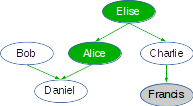
\includegraphics[width=120px]{family.png} \\
\hline
\end{tabular}

Alcune interrogazioni che \`e possibile effettuare con il conjunctive query 
answering sono:
\begin{itemize}
 \item ``Trova tutti gli individui maschi.''
 \item ``Chi sono gli individui con almeno un figlio maschio?''
 \item ``Chi sono i figli di $Alice$?''
 \item ``Chi sono gli individui con almeno un figlio maschio ed una femmina?''
 \item ``Chi sono gli individui maschi con almeno un figlio maschio?''
\end{itemize}
\end{frame}

\begin{frame}
\frametitle{Formule Atomiche}

Per definire in maniera rigorosa le query congiuntive \`e necessario
definire preliminarmente l'insieme delle \emph{formule atomiche}. 
\vspace{\baselineskip}

Sia $\VNames = \{x, y, z, ... \}$ l'insieme infinito, numerabile 
e disgiunto da $\CNames$, $\PNames$ e $\INames$ delle \emph{variabili}.
Le \emph{formule atomiche} sono espressioni dei due seguenti tipi:
\[
 C(\alpha), \quad P(\alpha, \beta)
\]
con $\alpha, \beta \in \INames \cup \VNames$, $C \in \CNames$ e $P \in \PNames$.
\vspace{\baselineskip}

Esempi di formule atomiche sono:
\begin{itemize}
 \item $HumanBeing(x)$,
 \item $x\,childOf\,Alice$,
 \item $Bob\,childOf\,x$,
 \item $x\,childOf\,y$,
 \item $Mortal(Socrate)$,
 \item $Alice\,childOf\,Elise$
\end{itemize}
con $HumanBeing, Mortal \in \CNames$, $childOf \in \PNames$, 
$Alice, Bob, Elise \in \INames$ e $x, y \in \VNames$.
\end{frame}

\begin{frame}
\frametitle{Formule Atomiche Chiuse}
Una formula atomica nella quale non compaiano variabili si dice \emph{chiusa}.
\vspace{\baselineskip}

Negli esempi che seguono sono evidenziate le formule atomiche chiuse:
\begin{itemize}
 \item $HumanBeing(x)$,
 \item $x\,childOf\,Alice$,
 \item $Bob\,childOf\,x$,
 \item $x\,childOf\,y$,
 \item $Mortal(Socrate)$,
 \item $Alice\,childOf\,Elise$
\end{itemize}
con $HumanBeing, Mortal \in \CNames$, $childOf \in \PNames$, 
$Alice, Bob, Elise \in \INames$ e $x, y \in \VNames$.
\vspace{\baselineskip}

\phantom{Le asserzioni presenti nelle ontologie sono formule atomiche chiuse.}
\end{frame}

\begin{frame}
\frametitle{Formule Atomiche Chiuse}
Una formula atomica nella quale non compaiano variabili si dice \emph{chiusa}.
\vspace{\baselineskip}

Negli esempi che seguono sono evidenziate le formule atomiche chiuse:
\begin{itemize}
 \item $HumanBeing(x)$,
 \item $x\,childOf\,Alice$,
 \item $Bob\,childOf\,x$,
 \item $x\,childOf\,y$,
 \item $\mathbf{Mortal(Socrate)}$,
 \item $\mathbf{Alice\,childOf\,Elise}$
\end{itemize}
con $HumanBeing, Mortal \in \CNames$, $childOf \in \PNames$, 
$Alice, Bob, Elise \in \INames$ e $x, y \in \VNames$.
\vspace{\baselineskip}

Le asserzioni presenti nelle ontologie sono formule atomiche chiuse.
\end{frame}

\begin{frame}
\frametitle{Query Congiuntive - }
Una \emph{query congiuntiva} \`e una congiunzione finita di formule atomiche $T_1 \wedge \ldots \wedge T_n$.
\vspace{\baselineskip}

Alcuni esempi di query congiuntive:
\begin{itemize}
 \item ``Trova tutti gli individui maschi.''
 \[
  Male(x)
 \]
 \item ``Chi sono gli individui con almeno un figlio maschio?''
\[
 y\,childOf\,x\,\wedge\,Male(y)  
\]
 \item ``Chi sono i figli di $Alice$?''
\[
 x\,childOf\,Alice
\]
%  \item ``Chi sono gli individui con almeno un figlio maschio ed una femmina?''
% \[
%  y\,childOf\,x\,\wedge\,Male(y)\,\wedge\,z\,childOf\,x\,\wedge\,Female(z)   
% \]
%  \item ``Chi sono gli individui maschi con almeno un figlio maschio?''
% \[
%  Male(x)\,\wedge\,y\,childOf\,x\,\wedge\,Male(y)
% \]
% con $x, y \in \VNames$, $Male, Female \in \CNames$, $childOf \in \PNames$ e $Alice \in \INames$.
 \end{itemize}
con $x, y \in \VNames$, $Male \in \CNames$, $childOf \in \PNames$ e $Alice \in
\INames$.
\end{frame}

\begin{frame}
\frametitle{Sostituzioni (1/2)}

Per definire le \emph{soluzioni} (risposte) delle query congiuntive introduciamo la
nozione di \emph{sostituzione}.
\vspace{\baselineskip}

Una \emph{sostituzione} $\sigma=[x_1 \rightarrow a_1, \ldots, x_n \rightarrow a_n]$
($x_1, \ldots, x_n \in \VNames$, $a_1, \ldots, a_n \in \INames$)
\`e una mappa finita che associa nomi di individui a variabili.
\vspace{\baselineskip}

Sia $T$ una formula atomica e $\sigma=[x_1 \rightarrow a_1, \ldots, x_n \rightarrow a_n]$
una sostituzione. L'\emph{applicazione} $T\sigma$ di $\sigma$ a $T$ \`e la formula atomica 
che si ottiene sostituendo in $T$ ad ogni occorrenza della variabile $x_i$ il
corrispondente nome di individuo $a_i$, per ogni $1\leq i\leq n$.
\vspace{\baselineskip}

Alcuni esempi:
\[
 \begin{array}{lcl}
  Male(x)[x \rightarrow Bob] & = & Male(Bob) \\
  Male(x)[y \rightarrow Bob] & = & \phantom{Male(x)} \\
  (x\,childOf\,y)[x \rightarrow Alice] & = & \phantom{Alice\,childOf\,y} \\
  (x\,childOf\,y)[x \rightarrow Alice, y \rightarrow Elise] & = & \phantom{Alice\,childOf\,Elise}
 \end{array}
\]
con $x,y \in \VNames$, $Male \in \CNames$, $childOf \in \PNames$ e $Alice, Bob, Elise \in \INames$.
\end{frame}

\begin{frame}
\frametitle{Sostituzioni (1/2)}

Per definire le \emph{soluzioni} (risposte) delle query congiuntive introduciamo la
nozione di \emph{sostituzione}.
\vspace{\baselineskip}

Una \emph{sostituzione} $\sigma=[x_1 \rightarrow a_1, \ldots, x_n \rightarrow a_n]$
($x_1, \ldots, x_n \in \VNames$, $a_1, \ldots, a_n \in \INames$)
\`e una mappa finita che associa nomi di individui a variabili.
\vspace{\baselineskip}

Sia $T$ una formula atomica e $\sigma=[x_1 \rightarrow a_1, \ldots, x_n \rightarrow a_n]$
una sostituzione. L'\emph{applicazione} $T\sigma$ di $\sigma$ a $T$ \`e la formula atomica 
che si ottiene sostituendo in $T$ ad ogni occorrenza della variabile $x_i$ il
corrispondente nome di individuo $a_i$, per ogni $1\leq i\leq n$.
\vspace{\baselineskip}

Alcuni esempi:
\[
 \begin{array}{lcl}
  Male(x)[x \rightarrow Bob] & = & Male(Bob) \\
  Male(x)[y \rightarrow Bob] & = & Male(x) \\
  (x\,childOf\,y)[x \rightarrow Alice] & = & \phantom{Alice\,childOf\,y} \\
  (x\,childOf\,y)[x \rightarrow Alice, y \rightarrow Elise] & = & \phantom{Alice\,childOf\,Elise}
 \end{array}
\]
con $x,y \in \VNames$, $Male \in \CNames$, $childOf \in \PNames$ e $Alice, Bob, Elise \in \INames$.
\end{frame}

\begin{frame}
\frametitle{Sostituzioni (1/2)}

Per definire le \emph{soluzioni} (risposte) delle query congiuntive introduciamo la
nozione di \emph{sostituzione}.
\vspace{\baselineskip}

Una \emph{sostituzione} $\sigma=[x_1 \rightarrow a_1, \ldots, x_n \rightarrow a_n]$
($x_1, \ldots, x_n \in \VNames$, $a_1, \ldots, a_n \in \INames$)
\`e una mappa finita che associa nomi di individui a variabili.
\vspace{\baselineskip}

Sia $T$ una formula atomica e $\sigma=[x_1 \rightarrow a_1, \ldots, x_n \rightarrow a_n]$
una sostituzione. L'\emph{applicazione} $T\sigma$ di $\sigma$ a $T$ \`e la formula atomica
che si ottiene sostituendo in $T$ ad ogni occorrenza della variabile $x_i$ il
corrispondente nome di individuo $a_i$, per ogni $1\leq i\leq n$.
\vspace{\baselineskip}

Alcuni esempi:
\[
 \begin{array}{lcl}
  Male(x)[x \rightarrow Bob] & = & Male(Bob) \\
  Male(x)[y \rightarrow Bob] & = & Male(x) \\
  (x\,childOf\,y)[x \rightarrow Alice] & = & Alice\,childOf\,y \\
  (x\,childOf\,y)[x \rightarrow Alice, y \rightarrow Elise] & = & \phantom{Alice\,childOf\,Elise}
 \end{array}
\]
con $x,y \in \VNames$, $Male \in \CNames$, $childOf \in \PNames$ e $Alice, Bob, Elise \in \INames$.
\end{frame}

\begin{frame}
\frametitle{Sostituzioni (1/2)}

Per definire le \emph{soluzioni} (risposte) delle query congiuntive introduciamo la
nozione di \emph{sostituzione}.
\vspace{\baselineskip}

Una \emph{sostituzione} $\sigma=[x_1 \rightarrow a_1, \ldots, x_n \rightarrow a_n]$
($x_1, \ldots, x_n \in \VNames$, $a_1, \ldots, a_n \in \INames$)
\`e una mappa finita che associa nomi di individui a variabili.
\vspace{\baselineskip}

Sia $T$ una formula atomica e $\sigma=[x_1 \rightarrow a_1, \ldots, x_n \rightarrow a_n]$
una sostituzione. L'\emph{applicazione} $T\sigma$ di $\sigma$ a $T$ \`e la formula atomica
che si ottiene sostituendo in $T$ ad ogni occorrenza della variabile $x_i$ il
corrispondente nome di individuo $a_i$, per ogni $1\leq i\leq n$.
\vspace{\baselineskip}

Alcuni esempi:
\[
 \begin{array}{lcl}
  Male(x)[x \rightarrow Bob] & = & Male(Bob) \\
  Male(x)[y \rightarrow Bob] & = & Male(x) \\
  (x\,childOf\,y)[x \rightarrow Alice] & = & Alice\,childOf\,y \\
  (x\,childOf\,y)[x \rightarrow Alice, y \rightarrow Elise] & = & Alice\,childOf\,Elise
 \end{array}
\]
con $x,y \in \VNames$, $Male \in \CNames$, $childOf \in \PNames$ e $Alice, Bob, Elise \in \INames$.
\end{frame}

\begin{frame}
\frametitle{Sostituzioni (2/2)}

L'applicazione di sostituzioni a query congiuntive si definisce come segue.
\vspace{\baselineskip}

Sia $\sigma=[x_1 \rightarrow a_1, \ldots, x_n \rightarrow a_n]$ una sostituzione
e siano $T_1, \ldots, T_m$ formule atomiche. Allora
\[
 (T_1 \wedge \ldots \wedge T_m)\sigma \defAs T_1\sigma \wedge \ldots \wedge T_m\sigma . 
\]
\vspace{\baselineskip}

Alcuni esempi:
\[
 \begin{array}{lcl}
 (y\,childOf\,x\,\wedge\,Male(y))[x \rightarrow Alice] & \defAs & \phantom{y\,childOf\,Alice\,\wedge\,Male(y)}  \\
 (y\,childOf\,x\,\wedge\,Male(y))[x \rightarrow Alice, z \rightarrow Bob] & \defAs & \phantom{y\,childOf\,Alice\,\wedge\,Male(y)}  \\
 (y\,childOf\,x\,\wedge\,Male(y))[x \rightarrow Alice, y \rightarrow Bob] & \defAs & \phantom{Bob\,childOf\,Alice\,\wedge\,Male(Bob)}  \\
 \end{array}
\]
\end{frame}

\begin{frame}
\frametitle{Sostituzioni (2/2)}

L'applicazione di sostituzioni a query congiuntive si definisce come segue.
\vspace{\baselineskip}

Sia $\sigma=[x_1 \rightarrow a_1, \ldots, x_n \rightarrow a_n]$ una sostituzione
e siano $T_1, \ldots, T_m$ formule atomiche. Allora
\[
 (T_1 \wedge \ldots \wedge T_m)\sigma \defAs T_1\sigma \wedge \ldots \wedge T_m\sigma . 
\]
\vspace{\baselineskip}

Alcuni esempi:
\[
 \begin{array}{lcl}
 (y\,childOf\,x\,\wedge\,Male(y))[x \rightarrow Alice] & \defAs & y\,childOf\,Alice\,\wedge\,Male(y)  \\
 (y\,childOf\,x\,\wedge\,Male(y))[x \rightarrow Alice, z \rightarrow Bob] & \defAs & \phantom{y\,childOf\,Alice\,\wedge\,Male(y)}  \\
 (y\,childOf\,x\,\wedge\,Male(y))[x \rightarrow Alice, y \rightarrow Bob] & \defAs & \phantom{Bob\,childOf\,Alice\,\wedge\,Male(Bob)}  \\
 \end{array}
\]
\end{frame}

\begin{frame}
\frametitle{Sostituzioni (2/2)}

L'applicazione di sostituzioni a query congiuntive si definisce come segue.
\vspace{\baselineskip}

Sia $\sigma=[x_1 \rightarrow a_1, \ldots, x_n \rightarrow a_n]$ una sostituzione
e siano $T_1, \ldots, T_m$ formule atomiche. Allora
\[
 (T_1 \wedge \ldots \wedge T_m)\sigma \defAs T_1\sigma \wedge \ldots \wedge T_m\sigma . 
\]
\vspace{\baselineskip}

Alcuni esempi:
\[
 \begin{array}{lcl}
 (y\,childOf\,x\,\wedge\,Male(y))[x \rightarrow Alice] & \defAs & y\,childOf\,Alice\,\wedge\,Male(y)  \\
 (y\,childOf\,x\,\wedge\,Male(y))[x \rightarrow Alice, z \rightarrow Bob] & \defAs & y\,childOf\,Alice\,\wedge\,Male(y)  \\
 (y\,childOf\,x\,\wedge\,Male(y))[x \rightarrow Alice, y \rightarrow Bob] & \defAs & \phantom{Bob\,childOf\,Alice\,\wedge\,Male(Bob)}  \\
 \end{array}
\]
\end{frame}

\begin{frame}
\frametitle{Sostituzioni (2/2)}

L'applicazione di sostituzioni a query congiuntive si definisce come segue.
\vspace{\baselineskip}

Sia $\sigma=[x_1 \rightarrow a_1, \ldots, x_n \rightarrow a_n]$ una sostituzione
e siano $T_1, \ldots, T_m$ formule atomiche. Allora
\[
 (T_1 \wedge \ldots \wedge T_m)\sigma \defAs T_1\sigma \wedge \ldots \wedge T_m\sigma . 
\]
\vspace{\baselineskip}

Alcuni esempi:
\[
 \begin{array}{lcl}
 (y\,childOf\,x\,\wedge\,Male(y))[x \rightarrow Alice] & \defAs & y\,childOf\,Alice\,\wedge\,Male(y)  \\
 (y\,childOf\,x\,\wedge\,Male(y))[x \rightarrow Alice, z \rightarrow Bob] & \defAs & y\,childOf\,Alice\,\wedge\,Male(y)  \\
 (y\,childOf\,x\,\wedge\,Male(y))[x \rightarrow Alice, y \rightarrow Bob] & \defAs & Bob\,childOf\,Alice\,\wedge\,Male(Bob)  \\
 \end{array}
\]
\end{frame}

\begin{frame}
\frametitle{Soluzioni per una Query}
Siano $\sigma=[x_1 \rightarrow a_1, \ldots, x_n \rightarrow a_n]$ una sostituzione,
$Q=T_1 \wedge \ldots \wedge T_m$ una query congiuntiva e $\Ont$ una ontologia.
\vspace{\baselineskip}

$\sigma$ \`e detta essere una \emph{soluzione} per $Q$ rispetto ad $\Ont$ se
e solo se 
\[
	\Ont \Longrightarrow T_i\sigma
\]
per ogni $1\leq i\leq m$. In altre parole, $T_i\sigma$ deve essere in $\Ont$ o
deve essere una conseguenza di $\Ont$, per ogni $T_i$ nella query.
\vspace{\baselineskip}

Consideriamo l'ontologia $\Ont$ e la query $Q$ definite come segue:
\[
\begin{array}{cl}
  \Ont  =  &  \{Female(Elise), Female(Alice), Male(Bob), \\
  &\phantom{\{}Male(Charlie), Male(Daniel), \\
  &\phantom{\{}Alice\,childOf\,Elise, Charlie\,childOf\,Elise, \\
  &\phantom{\{}Daniel\,childOf\,Alice, Daniel\,childOf\,Bob, \\
  &\phantom{\{}Francis\,childOf\,Charlie \}\\
  &\\
  Q = & y\,childOf\,x\,\wedge\,Male(y) .
 \end{array}
\]
Sia $\sigma_1=[x \rightarrow Alice, y \rightarrow Daniel]$. $\sigma_1$ \`e una soluzione per $Q$
rispetto ad $\Ont$?
\end{frame}

\begin{frame}
\frametitle{Soluzioni per una Query - Esempio 1}
Siano $\sigma=[x_1 \rightarrow a_1, \ldots, x_n \rightarrow a_n]$ una sostituzione,
$Q=T_1 \wedge \ldots \wedge T_m$ una query congiuntiva e $\Ont$ una ontologia.
\vspace{\baselineskip}

$\sigma$ \`e detta essere una \emph{soluzione} per $Q$ rispetto ad $\Ont$ se
e solo se $T_1\sigma, \ldots, T_2\sigma$ compaiono in $\Ont$. 
\vspace{\baselineskip}

Consideriamo l'ontologia $\Ont$ e la query $Q$ (``Chi sono gli individui con almeno un figlio maschio?'') definite come segue:
\[
\begin{array}{cl}
  \Ont  =  &  \{Female(Elise), Female(Alice), Male(Bob), \\
  &\phantom{\{}Male(Charlie), \textbf{Male(Daniel)}, \\
  &\phantom{\{}Alice\,childOf\,Elise, Charlie\,childOf\,Elise, \\
  &\phantom{\{}\textbf{Daniel\,childOf\,Alice}, Daniel\,childOf\,Bob, \\
  &\phantom{\{}Francis\,childOf\,Charlie \}\\
  &\\
  Q = & y\,childOf\,x\,\wedge\,Male(y) .
 \end{array}
\]
Sia $\sigma_1=[x \rightarrow Alice, y \rightarrow Daniel]$. $\sigma_1$ \`e una soluzione per $Q$
rispetto ad $\Ont$? \textbf{SI}.
\[
 Q\sigma_1 = Daniel\,childOf\,Alice\,\wedge\,Male(Daniel) .
\]
\end{frame}

\begin{frame}
\frametitle{Soluzioni per una Query - Esempio 2}
Siano $\sigma=[x_1 \rightarrow a_1, \ldots, x_n \rightarrow a_n]$ una sostituzione,
$Q=T_1 \wedge \ldots \wedge T_m$ una query congiuntiva e $\Ont$ una ontologia.
\vspace{\baselineskip}

$\sigma$ \`e detta essere una \emph{soluzione} per $Q$ rispetto ad $\Ont$ se
e solo se $T_1\sigma, \ldots, T_2\sigma$ compaiono in $\Ont$. 
\vspace{\baselineskip}

Consideriamo l'ontologia $\Ont$ e la query $Q$ definite come segue:
\[
\begin{array}{cl}
  \Ont  =  &  \{Female(Elise), Female(Alice), Male(Bob), \\
  &\phantom{\{}Male(Charlie), Male(Daniel), \\
  &\phantom{\{}Alice\,childOf\,Elise, Charlie\,childOf\,Elise, \\
  &\phantom{\{}Daniel\,childOf\,Alice, Daniel\,childOf\,Bob, \\
  &\phantom{\{}Francis\,childOf\,Charlie \}\\
  &\\
  Q = & y\,childOf\,x\,\wedge\,Male(y) .
 \end{array}
\]
Sia $\sigma_2=[x \rightarrow Alice, y \rightarrow Bob]$. $\sigma_2$ \`e una soluzione per $Q$
rispetto ad $\Ont$?
\end{frame}

\begin{frame}
\frametitle{Soluzioni per una Query - Esempio 2}
Siano $\sigma=[x_1 \rightarrow a_1, \ldots, x_n \rightarrow a_n]$ una sostituzione,
$Q=T_1 \wedge \ldots \wedge T_m$ una query congiuntiva e $\Ont$ una ontologia.
\vspace{\baselineskip}

$\sigma$ \`e detta essere una \emph{soluzione} per $Q$ rispetto ad $\Ont$ se
e solo se $T_1\sigma, \ldots, T_2\sigma$ compaiono in $\Ont$. 
\vspace{\baselineskip}

Consideriamo l'ontologia $\Ont$ e la query $Q$ (``Chi sono gli individui con almeno un figlio maschio?'') definite come segue:
\[
\begin{array}{cl}
  \Ont  =  &  \{Female(Elise), Female(Alice), Male(Bob), \\
  &\phantom{\{}Male(Charlie), Male(Daniel), \\
  &\phantom{\{}Alice\,childOf\,Elise, Charlie\,childOf\,Elise, \\
  &\phantom{\{}Daniel\,childOf\,Alice, Daniel\,childOf\,Bob, \\
  &\phantom{\{}Francis\,childOf\,Charlie \}\\
  &\\
  Q = & y\,childOf\,x\,\wedge\,Male(y) .
 \end{array}
\]
Sia $\sigma_2=[x \rightarrow Alice, y \rightarrow Bob]$. $\sigma_2$ \`e una soluzione per $Q$
rispetto ad $\Ont$? \textbf{NO}.
\[
 Q\sigma_2 = \mathbf{Bob\,childOf\,Alice}\,\wedge\,Male(Bob) .
\]
\end{frame}

\begin{frame}
\frametitle{Soluzioni per una Query - Esempio 3}
Siano $\sigma=[x_1 \rightarrow a_1, \ldots, x_n \rightarrow a_n]$ una sostituzione,
$Q=T_1 \wedge \ldots \wedge T_m$ una query congiuntiva e $\Ont$ una ontologia.
\vspace{\baselineskip}

$\sigma$ \`e detta essere una \emph{soluzione} per $Q$ rispetto ad $\Ont$ se
e solo se $T_1\sigma, \ldots, T_2\sigma$ compaiono in $\Ont$. 
\vspace{\baselineskip}

Consideriamo l'ontologia $\Ont$ e la query $Q$ definite come segue:
\[
\begin{array}{cl}
  \Ont  =  &  \{Female(Elise), Female(Alice), Male(Bob), \\
  &\phantom{\{}Male(Charlie), Male(Daniel), \\
  &\phantom{\{}Alice\,childOf\,Elise, Charlie\,childOf\,Elise, \\
  &\phantom{\{}Daniel\,childOf\,Alice, Daniel\,childOf\,Bob, \\
  &\phantom{\{}Francis\,childOf\,Charlie \}\\
  &\\
  Q = & y\,childOf\,x\,\wedge\,Male(y) .
 \end{array}
\]
Sia $\sigma_3=[x \rightarrow Charlie, y \rightarrow Francis]$. $\sigma_3$ \`e una soluzione per $Q$
rispetto ad $\Ont$?
\end{frame}

\begin{frame}
\frametitle{Soluzioni per una Query - Esempio 3}
Siano $\sigma=[x_1 \rightarrow a_1, \ldots, x_n \rightarrow a_n]$ una sostituzione,
$Q=T_1 \wedge \ldots \wedge T_m$ una query congiuntiva e $\Ont$ una ontologia.
\vspace{\baselineskip}

$\sigma$ \`e detta essere una \emph{soluzione} per $Q$ rispetto ad $\Ont$ se
e solo se $T_1\sigma, \ldots, T_2\sigma$ compaiono in $\Ont$. 
\vspace{\baselineskip}

Consideriamo l'ontologia $\Ont$ e la query $Q$ (``Chi sono gli individui con almeno un figlio maschio?'') definite come segue:
\[
\begin{array}{cl}
  \Ont  =  &  \{Female(Elise), Female(Alice), Male(Bob), \\
  &\phantom{\{}Male(Charlie), Male(Daniel), \\
  &\phantom{\{}Alice\,childOf\,Elise, Charlie\,childOf\,Elise, \\
  &\phantom{\{}Daniel\,childOf\,Alice, Daniel\,childOf\,Bob, \\
  &\phantom{\{}Francis\,childOf\,Charlie \}\\
  &\\
  Q = & y\,childOf\,x\,\wedge\,Male(y) .
 \end{array}
\]
Sia $\sigma_3=[x \rightarrow Charlie, y \rightarrow Francis]$. $\sigma_2$ \`e una soluzione per $Q$
rispetto ad $\Ont$? \textbf{NO}.
\[
 Q\sigma_3 = Francis\,childOf\,Charlie\,\wedge\,\mathbf{Male(Francis)} .
\]
\end{frame}

\begin{frame}
\frametitle{Soluzioni per una Query - Esempio 4}
Siano $\sigma=[x_1 \rightarrow a_1, \ldots, x_n \rightarrow a_n]$ una sostituzione,
$Q=T_1 \wedge \ldots \wedge T_m$ una query congiuntiva e $\Ont$ una ontologia.
\vspace{\baselineskip}

$\sigma$ \`e detta essere una \emph{soluzione} per $Q$ rispetto ad $\Ont$ se
e solo se $T_1\sigma, \ldots, T_2\sigma$ compaiono in $\Ont$. 
\vspace{\baselineskip}

Consideriamo l'ontologia $\Ont$ e la query $Q$ definite come segue:
\[
\begin{array}{cl}
  \Ont  =  &  \{Female(Elise), Female(Alice), Male(Bob), \\
  &\phantom{\{}Male(Charlie), Male(Daniel), \\
  &\phantom{\{}Alice\,childOf\,Elise, Charlie\,childOf\,Elise, \\
  &\phantom{\{}Daniel\,childOf\,Alice, Daniel\,childOf\,Bob, \\
  &\phantom{\{}Francis\,childOf\,Charlie \}\\
  &\\
  Q = & y\,childOf\,x\,\wedge\,Male(y) .
 \end{array}
\]
Sia $\sigma_4=[y \rightarrow Daniel]$. $\sigma_4$ \`e una soluzione per $Q$
rispetto ad $\Ont$?
\phantom{Affinch\`e una sostituzione $\sigma$ sia una soluzione per una query $Q$
(a prescindere dall'ontologia) \`e necessario che in $\sigma$ compaiano
tutte le variabili di $Q$.}
\end{frame}

\begin{frame}
\frametitle{Soluzioni per una Query - Esempio 4}
Siano $\sigma=[x_1 \rightarrow a_1, \ldots, x_n \rightarrow a_n]$ una sostituzione,
$Q=T_1 \wedge \ldots \wedge T_m$ una query congiuntiva e $\Ont$ una ontologia.
\vspace{\baselineskip}

$\sigma$ \`e detta essere una \emph{soluzione} per $Q$ rispetto ad $\Ont$ se
e solo se $T_1\sigma, \ldots, T_2\sigma$ compaiono in $\Ont$. 
\vspace{\baselineskip}

Consideriamo l'ontologia $\Ont$ e la query $Q$ (``Chi sono gli individui con almeno un figlio maschio?'') definite come segue:
\[
\begin{array}{cl}
  \Ont  =  &  \{Female(Elise), Female(Alice), Male(Bob), \\
  &\phantom{\{}Male(Charlie), Male(Daniel), \\
  &\phantom{\{}Alice\,childOf\,Elise, Charlie\,childOf\,Elise, \\
  &\phantom{\{}Daniel\,childOf\,Alice, Daniel\,childOf\,Bob, \\
  &\phantom{\{}Francis\,childOf\,Charlie \}\\
  &\\
  Q = & y\,childOf\,x\,\wedge\,Male(y) .
 \end{array}
\]
Sia $\sigma_4=[y \rightarrow Daniel]$. $\sigma_2$ \`e una soluzione per $Q$
rispetto ad $\Ont$? \textbf{NO}.
\[
 Q\sigma_4 = \mathbf{Daniel\,childOf\,x}\,\wedge\,Male(Daniel) .
\]
Affinch\`e una sostituzione $\sigma$ sia una soluzione per una query $Q$
(a prescindere dall'ontologia) \`e necessario che in $\sigma$ compaiano
tutte le variabili di $Q$.
\end{frame}

\begin{frame}
\frametitle{Soluzioni per una Query - Esempio 5}
Siano $\sigma=[x_1 \rightarrow a_1, \ldots, x_n \rightarrow a_n]$ una sostituzione,
$Q=T_1 \wedge \ldots \wedge T_m$ una query congiuntiva e $\Ont$ una ontologia.
\vspace{\baselineskip}

$\sigma$ \`e detta essere una \emph{soluzione} per $Q$ rispetto ad $\Ont$ se
e solo se $T_1\sigma, \ldots, T_2\sigma$ compaiono in $\Ont$. 
\vspace{\baselineskip}

Consideriamo l'ontologia $\Ont$ e la query $Q$ definite come segue:
\[
\begin{array}{cl}
  \Ont  =  &  \{Female(Elise), Female(Alice), Male(Bob), \\
  &\phantom{\{}Male(Charlie), Male(Daniel), \\
  &\phantom{\{}Alice\,childOf\,Elise, Charlie\,childOf\,Elise, \\
  &\phantom{\{}Daniel\,childOf\,Alice, Daniel\,childOf\,Bob, \\
  &\phantom{\{}Francis\,childOf\,Charlie \}\\
  &\\
  Q = & y\,childOf\,x\,\wedge\,Male(y) .
 \end{array}
\]
Sia $\sigma_5=[x \rightarrow Elise, y \rightarrow Charlie, z \rightarrow Francis]$. $\sigma_5$ \`e una soluzione per $Q$
rispetto ad $\Ont$?
\end{frame}

\begin{frame}
\frametitle{Soluzioni per una Query - Esempio 5}
Siano $\sigma=[x_1 \rightarrow a_1, \ldots, x_n \rightarrow a_n]$ una sostituzione,
$Q=T_1 \wedge \ldots \wedge T_m$ una query congiuntiva e $\Ont$ una ontologia.
\vspace{\baselineskip}

$\sigma$ \`e detta essere una \emph{soluzione} per $Q$ rispetto ad $\Ont$ se
e solo se $T_1\sigma, \ldots, T_2\sigma$ compaiono in $\Ont$. 
\vspace{\baselineskip}

Consideriamo l'ontologia $\Ont$ e la query $Q$ (``Chi sono gli individui con almeno un figlio maschio?'') definite come segue:
\[
\begin{array}{cl}
  \Ont  =  &  \{Female(Elise), Female(Alice), Male(Bob), \\
  &\phantom{\{}\mathbf{Male(Charlie)}, Male(Daniel), \\
  &\phantom{\{}Alice\,childOf\,Elise, \mathbf{Charlie\,childOf\,Elise}, \\
  &\phantom{\{}Daniel\,childOf\,Alice, Daniel\,childOf\,Bob, \\
  &\phantom{\{}Francis\,childOf\,Charlie \}\\
  &\\
  Q = & y\,childOf\,x\,\wedge\,Male(y) .
 \end{array}
\]
Sia $\sigma_5=[x \rightarrow Elise, y \rightarrow Charlie, z \rightarrow Francis]$. $\sigma_5$ \`e una soluzione per $Q$
rispetto ad $\Ont$? \textbf{SI}.
\[
 Q\sigma_5 = Charlie\,childOf\,Elise\,\wedge\,Male(Charlie) .
\]
\end{frame}

\begin{frame}
\frametitle{Soluzioni Minimali per una Query}
Siano $\sigma=[x_1 \rightarrow a_1, \ldots, x_n \rightarrow a_n]$ 
una sostituzione, $Q$ una query congiuntiva e $\Ont$ una ontologia.
\vspace{\baselineskip}

$\sigma$ \`e una \emph{soluzione minimale} per $Q$ rispetto a $\Ont$
se e solo se:
\begin{enumerate}
 \item $\sigma$ \`e una soluzione per $Q$ rispetto ad $\Ont$ e inoltre
 \item tutte le variabili $x_1, \ldots, x_n$ che compaiono in $\sigma$
 compaiono anche in $Q$ (criterio di minimalit\`a).
\end{enumerate}
Consideriamo ad esempio
\[
\begin{array}{cl}
  \Ont  =  &  \{Female(Elise), Female(Alice), Male(Bob), \\
  &\phantom{\{}Male(Charlie), Male(Daniel), \\
  &\phantom{\{}Alice\,childOf\,Elise, Charlie\,childOf\,Elise, \\
  &\phantom{\{}Daniel\,childOf\,Alice, Daniel\,childOf\,Bob, \\
  &\phantom{\{}Francis\,childOf\,Charlie \}\\
  &\\
  Q = & y\,childOf\,x\,\wedge\,Male(y) .
 \end{array}
\]
$\sigma_5=[x \rightarrow Elise, y \rightarrow Charlie, z \rightarrow Francis]$ \`e una 
soluzione minimale per $Q$ rispetto a $\Ont$? \phantom{\textbf{NO}.}
\vspace{\baselineskip}

\phantom{$\sigma_6=[x \rightarrow Elise, y \rightarrow Charlie]$ \`e una 
soluzione minimale per $Q$ rispetto a $\Ont$? \textbf{SI}.}
\end{frame}

\begin{frame}
\frametitle{Soluzioni Minimali per una Query}
Siano $\sigma=[x_1 \rightarrow a_1, \ldots, x_n \rightarrow a_n]$ 
una sostituzione, $Q$ una query congiuntiva e $\Ont$ una ontologia.
\vspace{\baselineskip}

$\sigma$ \`e una \emph{soluzione minimale} per $Q$ rispetto a $\Ont$
se e solo se:
\begin{enumerate}
 \item $\sigma$ \`e una soluzione per $Q$ rispetto ad $\Ont$ e inoltre
 \item tutte le variabili $x_1, \ldots, x_n$ che compaiono in $\sigma$
 compaiono anche in $Q$ (criterio di minimalit\`a).
\end{enumerate}
Consideriamo ad esempio
\[
\begin{array}{cl}
  \Ont  =  &  \{Female(Elise), Female(Alice), Male(Bob), \\
  &\phantom{\{}Male(Charlie), Male(Daniel), \\
  &\phantom{\{}Alice\,childOf\,Elise, Charlie\,childOf\,Elise, \\
  &\phantom{\{}Daniel\,childOf\,Alice, Daniel\,childOf\,Bob, \\
  &\phantom{\{}Francis\,childOf\,Charlie \}\\
  &\\
  Q = & y\,childOf\,x\,\wedge\,Male(y) .
 \end{array}
\]
$\sigma_5=[x \rightarrow Elise, y \rightarrow Charlie, \mathbf{z} \rightarrow Francis]$ \`e una 
soluzione minimale per $Q$ rispetto a $\Ont$? \textbf{NO}.
\vspace{\baselineskip}

$\sigma_6=[x \rightarrow Elise, y \rightarrow Charlie]$ \`e una 
soluzione minimale per $Q$ rispetto a $\Ont$? \phantom{\textbf{SI}}.
\end{frame}

\begin{frame}
\frametitle{Soluzioni Minimali per una Query}
Siano $\sigma=[x_1 \rightarrow a_1, \ldots, x_n \rightarrow a_n]$ 
una sostituzione, $Q$ una query congiuntiva e $\Ont$ una ontologia.
\vspace{\baselineskip}

$\sigma$ \`e una \emph{soluzione minimale} per $Q$ rispetto a $\Ont$
se e solo se:
\begin{enumerate}
 \item $\sigma$ \`e una soluzione per $Q$ rispetto ad $\Ont$ e inoltre
 \item tutte le variabili $x_1, \ldots, x_n$ che compaiono in $\sigma$
 compaiono anche in $Q$ (criterio di minimalit\`a).
\end{enumerate}
Consideriamo ad esempio
\[
\begin{array}{cl}
  \Ont  =  &  \{Female(Elise), Female(Alice), Male(Bob), \\
  &\phantom{\{}Male(Charlie), Male(Daniel), \\
  &\phantom{\{}Alice\,childOf\,Elise, Charlie\,childOf\,Elise, \\
  &\phantom{\{}Daniel\,childOf\,Alice, Daniel\,childOf\,Bob, \\
  &\phantom{\{}Francis\,childOf\,Charlie \}\\
  &\\
  Q = & y\,childOf\,x\,\wedge\,Male(y) .
 \end{array}
\]
$\sigma_5=[x \rightarrow Elise, y \rightarrow Charlie, \mathbf{z} \rightarrow Francis]$ \`e una 
soluzione minimale per $Q$ rispetto a $\Ont$? \textbf{NO}.
\vspace{\baselineskip}

$\sigma_6=[x \rightarrow Elise, y \rightarrow Charlie]$ \`e una 
soluzione minimale per $Q$ rispetto a $\Ont$? \textbf{SI}.
\end{frame}

\begin{frame}
\frametitle{Conjunctive Query Answering}
Il problema del \emph{Conjunctive Query Answering} consiste nel trovare
tutte le soluzioni minimali di una query congiuntiva rispetto ad una ontologia.
\vspace{\baselineskip}

Esse sono sempre in numero finito, infatti:
\begin{itemize}
 \item le variabili che compaiono nelle soluzioni sono esattamente quelle che compaiono nella query,
 \item i nomi di individui che compaiono nelle soluzioni sono un sottoinsieme di quelli che compaiono
 nell'ontologia.
\end{itemize}
\end{frame}

\begin{frame}
\frametitle{Conjunctive Query Answering}
Il problema del \emph{Conjunctive Query Answering} consiste nel trovare
tutte le soluzioni minimali di una query congiuntiva rispetto ad una ontologia.
\vspace{\baselineskip}

\begin{center}
Esempio 1:``Trova tutti gli individui maschi.'' 
\end{center}
%\vspace{\baselineskip}

\begin{tabular}{lc}
$\begin{array}{cl}
  \Ont  =  &  \{Female(Elise),  Female(Alice), Male(Bob), \\
  &\phantom{\{}Male(Charlie), Male(Daniel), \\
  &\phantom{\{}Alice\,childOf\,Elise, Charlie\,childOf\,Elise, \\
  &\phantom{\{}Daniel\,childOf\,Alice, Daniel\,childOf\,Bob, \\
  &\phantom{\{}Francis\,childOf\,Charlie \}\\
\end{array}$ &   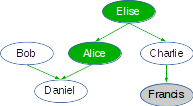
\includegraphics[width=130px]{family.png} \\
 $Q=Male(x)$ &
 $\begin{array}{|c|}
  \hline
  x\\
  \hline
  Bob\\
  Charlie\\
  Daniel\\
  \hline
\end{array}$ \\
\end{tabular}
\end{frame}


\begin{frame}
\frametitle{Conjunctive Query Answering - Esempio 2}
\begin{center}
``Chi sono gli individui con almeno un figlio maschio?'' 
\end{center}

\begin{tabular}{lc}
$\begin{array}{cl}
  \Ont  =  &  \{Female(Elise),  Female(Alice), Male(Bob), \\
  &\phantom{\{}Male(Charlie), Male(Daniel), \\
  &\phantom{\{}Alice\,childOf\,Elise, Charlie\,childOf\,Elise, \\
  &\phantom{\{}Daniel\,childOf\,Alice, Daniel\,childOf\,Bob, \\
  &\phantom{\{}Francis\,childOf\,Charlie \}\\
\end{array}$ &   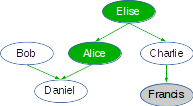
\includegraphics[width=130px]{family.png} \\
 $Q=y\,childOf\,x\,\wedge\,Male(y)$ &
$\begin{array}{|c|c|}
  \hline
  x & y\\
  \hline
  Elise&Charlie\\
  Alice&Daniel\\
  Bob&Daniel\\
  \hline
\end{array}$\\
\end{tabular}
\end{frame}


\begin{frame}
\frametitle{Conjunctive Query Answering - Esempio 3}
\begin{center}
``Chi sono i figli di $Elise$?''
\end{center}

\begin{tabular}{lc}
$\begin{array}{cl}
  \Ont  =  &  \{Female(Elise),  Female(Alice), Male(Bob), \\
  &\phantom{\{}Male(Charlie), Male(Daniel), \\
  &\phantom{\{}Alice\,childOf\,Elise, Charlie\,childOf\,Elise, \\
  &\phantom{\{}Daniel\,childOf\,Alice, Daniel\,childOf\,Bob, \\
  &\phantom{\{}Francis\,childOf\,Charlie \}\\
\end{array}$ & 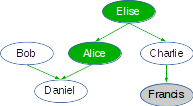
\includegraphics[width=130px]{family.png} \\
$Q=x\,childOf\,Elise$ &
$\begin{array}{|c|}
  \hline
  x\\
  \hline
  \phantom{Alice}\\
  \phantom{Charlie}\\
  \hline
\end{array}$ \\
\end{tabular}
\end{frame}

\begin{frame}
\frametitle{Conjunctive Query Answering - Esempio 3}
\begin{center}
``Chi sono i figli di $Elise$?''
\end{center}

\begin{tabular}{lc}
$\begin{array}{cl}
  \Ont  =  &  \{Female(Elise),  Female(Alice), Male(Bob), \\
  &\phantom{\{}Male(Charlie), Male(Daniel), \\
  &\phantom{\{}Alice\,childOf\,Elise, Charlie\,childOf\,Elise, \\
  &\phantom{\{}Daniel\,childOf\,Alice, Daniel\,childOf\,Bob, \\
  &\phantom{\{}Francis\,childOf\,Charlie \}\\
\end{array}$ & 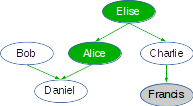
\includegraphics[width=130px]{family.png} \\
$Q=x\,childOf\,Elise$ &
$\begin{array}{|c|}
  \hline
  x\\
  \hline
  Alice\\
  Charlie\\
  \hline
\end{array}$ \\
\end{tabular}
\end{frame}

\begin{frame}
\frametitle{Conjunctive Query Answering - Esempio 4}
\begin{center}
``Chi sono gli individui con almeno un figlio maschio ed una femmina?''
\end{center}

\begin{tabular}{lc}
$\begin{array}{cl}
  \Ont  =  &  \{Female(Elise),  Female(Alice), Male(Bob), \\
  &\phantom{\{}Male(Charlie), Male(Daniel), \\
  &\phantom{\{}Alice\,childOf\,Elise, Charlie\,childOf\,Elise, \\
  &\phantom{\{}Daniel\,childOf\,Alice, Daniel\,childOf\,Bob, \\
  &\phantom{\{}Francis\,childOf\,Charlie \}\\
\end{array}$ & 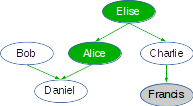
\includegraphics[width=130px]{family.png} \\
$\phantom{Q=y\,childOf\,x\,\wedge\,z\,childOf\,x\,\wedge\,Male(y)\,\wedge\,Female(z)}$ &
$\begin{array}{|c|c|c|}
  \hline
  x&y&z\\
  \hline
  \phantom{Elise}&\phantom{Charlie}&\phantom{Alice}\\
  \hline
\end{array}$ \\
\end{tabular}
\end{frame}

\begin{frame}
\frametitle{Conjunctive Query Answering - Esempio 4}
\begin{center}
``Chi sono gli individui con almeno un figlio maschio ed una femmina?''
\end{center}

\begin{tabular}{lc}
$\begin{array}{cl}
  \Ont  =  &  \{Female(Elise),  Female(Alice), Male(Bob), \\
  &\phantom{\{}Male(Charlie), Male(Daniel), \\
  &\phantom{\{}Alice\,childOf\,Elise, Charlie\,childOf\,Elise, \\
  &\phantom{\{}Daniel\,childOf\,Alice, Daniel\,childOf\,Bob, \\
  &\phantom{\{}Francis\,childOf\,Charlie \}\\
\end{array}$ & 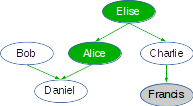
\includegraphics[width=130px]{family.png} \\
$Q=y\,childOf\,x\,\wedge\,z\,childOf\,x\,\wedge\,Male(y)\,\wedge\,Female(z)$ &
$\begin{array}{|c|c|c|}
  \hline
  x&y&z\\
  \hline
  \phantom{Elise}&\phantom{Charlie}&\phantom{Alice}\\
  \hline
\end{array}$ \\
\end{tabular}
\end{frame}

\begin{frame}
\frametitle{Conjunctive Query Answering - Esempio 4}
\begin{center}
``Chi sono gli individui con almeno un figlio maschio ed una femmina?''
\end{center}

\begin{tabular}{lc}
$\begin{array}{cl}
  \Ont  =  &  \{Female(Elise),  Female(Alice), Male(Bob), \\
  &\phantom{\{}Male(Charlie), Male(Daniel), \\
  &\phantom{\{}Alice\,childOf\,Elise, Charlie\,childOf\,Elise, \\
  &\phantom{\{}Daniel\,childOf\,Alice, Daniel\,childOf\,Bob, \\
  &\phantom{\{}Francis\,childOf\,Charlie \}\\
\end{array}$ & 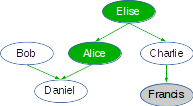
\includegraphics[width=130px]{family.png} \\
$Q=y\,childOf\,x\,\wedge\,z\,childOf\,x\,\wedge\,Male(y)\,\wedge\,Female(z)$ &
$\begin{array}{|c|c|c|}
  \hline
  x&y&z\\
  \hline
  Elise&Charlie&Alice\\
  \hline
\end{array}$ \\
\end{tabular}
\end{frame}


\begin{frame}
\frametitle{Conjunctive Query Answering - Esempio 5}
\begin{center}
``Chi sono gli individui maschi con almeno una figlia femmina?''
\end{center}

\begin{tabular}{lc}
$\begin{array}{cl}
  \Ont  =  &  \{Female(Elise), Female(Alice), Male(Bob), \\
  &\phantom{\{}Male(Charlie), Male(Daniel), \\
  &\phantom{\{}Alice\,childOf\,Elise, Charlie\,childOf\,Elise, \\
  &\phantom{\{}Daniel\,childOf\,Alice, Daniel\,childOf\,Bob, \\
  &\phantom{\{}Francis\,childOf\,Charlie \}\\
\end{array}$ & 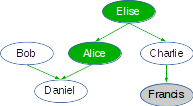
\includegraphics[width=130px]{family.png} \\
$\phantom{Q=Male(x)\,\wedge\,y\,childOf\,x\,\wedge\,Female(y)}$ &
$\begin{array}{|c|c|}
  \hline
  x&y\\
  \hline
  &\\
  &\\
  \hline
\end{array}$\\
\end{tabular}
\end{frame}

\begin{frame}
\frametitle{Conjunctive Query Answering - Esempio 5}
\begin{center}
``Chi sono gli individui maschi con almeno una figlia femmina?''
\end{center}

\begin{tabular}{lc}
$\begin{array}{cl}
  \Ont  =  &  \{Female(Elise), Female(Alice), Male(Bob), \\
  &\phantom{\{}Male(Charlie), Male(Daniel), \\
  &\phantom{\{}Alice\,childOf\,Elise, Charlie\,childOf\,Elise, \\
  &\phantom{\{}Daniel\,childOf\,Alice, Daniel\,childOf\,Bob, \\
  &\phantom{\{}Francis\,childOf\,Charlie \}\\
\end{array}$ & 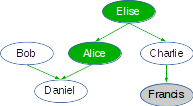
\includegraphics[width=130px]{family.png} \\
$Q=Male(x)\,\wedge\,y\,childOf\,x\,\wedge\,Female(y)$ &
$\begin{array}{|c|c|}
  \hline
  x&y\\
  \hline
  &\\
  &\\
  \hline
\end{array}$\\
\end{tabular}
\end{frame}

\begin{frame}
\frametitle{Conjunctive Query Answering - Esempio 5}
\begin{center}
``Chi sono gli individui maschi con almeno una figlia femmina?''
\end{center}

\begin{tabular}{lc}
$\begin{array}{cl}
  \Ont  =  &  \{Female(Elise), Female(Alice), Male(Bob), \\
  &\phantom{\{}Male(Charlie), Male(Daniel), \\
  &\phantom{\{}Alice\,childOf\,Elise, Charlie\,childOf\,Elise, \\
  &\phantom{\{}Daniel\,childOf\,Alice, Daniel\,childOf\,Bob, \\
  &\phantom{\{}Francis\,childOf\,Charlie \}\\
\end{array}$ & 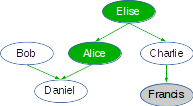
\includegraphics[width=130px]{family.png} \\
$Q=Male(x)\,\wedge\,y\,childOf\,x\,\wedge\,Female(y)$ & Nessuna soluzione\\
\end{tabular}
\end{frame}

% 
% 
% \begin{frame}
% \frametitle{Vocabolari condivisi}
% 
% L'utilizzo di vocabolari condivisi (ben noti) favorisce la 
% scalabilit\`a orizzontale delle applicazioni. 
% \vspace{\baselineskip}
% 
% Ad esempio, una 
% applicazione sviluppata sull'ontologia di un comune che utilizzi 
% i vocabolari standard per le pubbliche amministrazioni (vedi le \emph{Linee 
% Guida per la Valorizzazione del Patrimonio Informativo Pubblico} dell'\emph{Agenzia per l'Italia Digitale}) 
% pu\`o essere estesa senza sforzi aggiuntivi per utilizzare i dati provenienti
% dalle ontologie di tutti i comuni.
% \end{frame}
% 
% 
% \begin{frame}
% \frametitle{Il Vocabolario FOAF}
% Uno dei primi e pi\`u utilizzati vocabolari definiti nell'ambito
% del Web semantico \`e \emph{Friend OF A Friend} (\emph{FOAF}, vedi \url{http://foaf-project.org}).
% \vspace{\baselineskip}
% 
% 
% \begin{quote}
% FOAF is a project devoted to linking people and information using the Web. 
% \end{quote}
% 
% In questa sede ci limiteremo solo alla parte \emph{Core}.
% \begin{quote}
% \textbf{Core} - These classes and properties form the core of FOAF. They
% describe characteristics of people and social groups that are
% independent of time and technology; as such they can be used to
% describe basic information about people in present day, historical,
% cultural heritage and digital library contexts. In addition to various
% characteristics of people, FOAF defines classes for Project,
% Organization and Group as other kinds of agent. Related work: 
% \end{quote}
% (tratto da \emph{FOAF Vocabulary Specification 0.99},
% Namespace Document 14 January 2014, Paddington Edition, \url{http://xmlns.com/foaf/spec/})
% \end{frame}
% 
% \newcommand{\foafcore}{\mathtt{FOAFCore}}
% \begin{frame}
% \frametitle{FOAF Core}
% Il vocabolario \emph{Foaf Core} \`e definito come segue:
% \[
%  \begin{array}{ccl}
%  \foafcore & \defAs & (C_{foaf}, P_{foaf}, \Omega_{foaf}) \\
%  &&\\
%  C_{foaf} & \defAs & \{Agent, Person, Project, Organization, Group, Document, Image\}\\
%  &&\\
%  P_{foaf} & \defAs & \{name, title, img, depiction, depicts, familyName, givenName,\\
%  && \phantom{\}}, based\_near, age, made, maker, primaryTopic, primaryTopicOf, member \}\\
%  \Omega_{foaf} & \defAs & \{ Person \Issub Agent, Group \Issub Agent, Organization \Issub Agent, \\
%  && \phantom{\{} Image \Issub Document, \dom(title) \Issub Document, \\
%  && \phantom{\{}\range(depiction) \Issub Image, img \Issub depiction, \dom(img) \Issub Person,\\
%  && \phantom{\{}\dom(knows) \Issub Person, \range(knows) \Issub Person, \ldots \}\\
%  \end{array}
% \]
% \end{frame}
% 
% \begin{frame}
% \frametitle{Descrizioni Intuitive degli Elementi dei Vocabolari}
% Le classi e le propriet\`a di un vocabolario vengono spesso fornite
% di una descrizione intuitiva nel documento che descrive il vocabolario.
% Ad esempio, le classi $Agent$ e $Person$ vengono descritte come segue 
% in \url{http://xmlns.com/foaf/spec/}
% \begin{quote}
% \textbf{Agent} - The Agent class is the class of agents; things that do stuff. A well known 
% sub-class is Person, representing people. Other kinds of agents include 
% Organization and Group.
% 
% The Agent class is useful in a few places in FOAF where Person would have 
% been overly specific. For example, the IM chat ID properties such as 
% jabberID are typically associated with people, but sometimes belong to 
% software bots.  
% \end{quote}
% 
% \begin{quote}
% \textbf{Person} - The Person class represents people. Something is a Person if it is a person.
% We don't nitpic about whether they're alive, dead, real, or imaginary. 
% The Person class is a sub-class of the Agent class, since all people are 
% considered 'agents' in FOAF.  
% \end{quote}
% \end{frame}
% 
% \begin{frame}
% \frametitle{Descrizioni Rigorose degli Elementi dei Vocabolari}
% Tuttavia, gi\`a nei vincoli di un vocabolario si trovano indicazioni importanti
% sulla \emph{semantica} dei nomi di classe e di propriet\`a del vocabolario stesso.
% \[
% \begin{array}{l}
% Person \Issub Agent\\
% \range(depiction) \Issub Image\\
% img \Issub depiction, \\
% \dom(img) \Issub Person,\\
% \dom(knows) \Issub Person,\\
% \range(knows) \Issub Person,\\
% \ldots
% \end{array}
% \]
% \end{frame}
% 
% \begin{frame}
% \frametitle{Vocabolari Compositi}
% 
% \`E possibile costruire un vocabolario \emph{estendendone} un'altro.
% Ad esempio, il vocabolario \emph{Organization Ontology} (in breve \emph{ORG}, vedi \url{http://www.w3.org/TR/vocab-org/})
% estende FOAF con classi e propriet\`a, per modellare in dettaglio 
% le strutture organizzative di aziende, associazioni e tutte le forme 
% di organizzazioni.
% \vspace{\baselineskip}
% 
% Formalmente, dati due vocabolari
% \[
%  \begin{array}{lcl}
%  V & \defAs & (C, P, \Omega) \\ 
%  V' & \defAs & (C', P', \Omega')
%  \end{array}
% \]
% si dice che $V'$ \emph{importa} (o \emph{estende}) $V$ se e 
% solo se
% \[
%  \begin{array}{rcl}
%  C & \subseteq & C' \\
%  P & \subseteq & P' \\
%  \Omega & \subseteq & \Omega'  
% \end{array} 
% \]
% \end{frame}
% 
% \newcommand{\org}{\mathtt{ORG}}
% 
% \begin{frame}
% \frametitle{Il Vocabolario Organization Ontology}
% \emph{Organization Ontology},in breve \emph{ORG},\footnote{\url{http://www.w3.org/TR/vocab-org/}}
% estende FOAF con classi e propriet\`a, per modellare in dettaglio 
% le strutture organizzative di aziende, associazioni e tutte le forme 
% di organizzazioni.
% \vspace{\baselineskip}
% 
% \uncover<2->{
% Il vocabolario \`e disponibile alle URL
% \begin{center}
%   \url{http://www.w3.org/ns/org.rdf}
% \end{center}
% 
% \begin{center}
%   \url{http://www.w3.org/ns/org.ttl}
% \end{center}
% }
% 
% \uncover<3->{
% Il namespace del vocabolario ORG \`e
% \begin{center}
%   \url{org} : \url{http://www.w3.org/ns/org\#}
% \end{center}
% }
% 
% \[
%  \begin{array}{ccl}
%  \org & \defAs & (C_{org}, P_{org}, \Omega_{org}) \\
%  &&\\
%  C_{org} & \defAs & C_{foaf} \cup \{FormalOrganization, OrganizationalUnit,  Site \\
%  && \phantom{C_{foaf} \cup \{}Post, Role, \ldots \}\\
%  &&\\
%  P_{org} & \defAs & P_{foaf} \cup \{ basedAt, classification, hasPost, hasPrimarySite, \\
%  &&\phantom{P_{foaf} \cup \{}hasRegisteredSite, hasSite, hasSubOrganization, \\
%  &&\phantom{P_{foaf} \cup \{}hasUnit, headOf, heldBy, holds, location, postIn,\\
%  &&\phantom{P_{foaf} \cup \{}purpose, role, siteAddress, siteOf, unitOf, \\
%  &&\phantom{P_{foaf} \cup \{}subOrganizationOf,  transitiveSubOrganizationOf, \ldots \}\\
%  &&\phantom{P_{foaf} \cup \{}  \\
%  &&\\
%  \Omega_{org} & \defAs & \Omega_{foaf} \cup \{ FormalOrganization \Issub Organization, \\
%  &&\phantom{\Omega_{foaf} \cup \{}OrganizationalUnit \Issub Organization,\\
%  &&\phantom{\Omega_{foaf} \cup \{}headOf \Issub member, \dom(hasUnit)\Issub Organization, \\
%  &&\phantom{\Omega_{foaf} \cup \{}\range(hasUnit) \Issub OrganizationalUnit, \ldots \}
%  \end{array}
% \]
% \phantom{NOTA: I vincoli semantici esplicitano la relazione tra i due vocabolari.}
% \end{frame}
% 
% \begin{frame}
% \frametitle{Il Vocabolario Organization Ontology}
% Ad esempio, il vocabolario \emph{Organization Ontology} (in breve \emph{ORG}, vedi \url{http://www.w3.org/TR/vocab-org/})
% estende FOAF con classi e propriet\`a, per modellare in dettaglio 
% le strutture organizzative di aziende, associazioni e tutte le forme 
% di organizzazioni.
% 
% \[
%  \begin{array}{ccl}
%  \org & \defAs & (C_{org}, P_{org}, \Omega_{org}) \\
%  &&\\
%  C_{org} & \defAs & C_{foaf} \cup \{FormalOrganization, OrganizationalUnit,  Site \\
%  && \phantom{C_{foaf} \cup \{}Post, Role, \ldots \}\\
%  &&\\
%  P_{org} & \defAs & P_{foaf} \cup \{ basedAt, classification, hasPost, hasPrimarySite, \\
%  &&\phantom{P_{foaf} \cup \{}hasRegisteredSite, hasSite, hasSubOrganization, \\
%  &&\phantom{P_{foaf} \cup \{}hasUnit, headOf, heldBy, holds, location, postIn,\\
%  &&\phantom{P_{foaf} \cup \{}purpose, role, siteAddress, siteOf, unitOf, \\ 
%  &&\phantom{P_{foaf} \cup \{}subOrganizationOf,  transitiveSubOrganizationOf, \ldots \}\\ 
%  &&\phantom{P_{foaf} \cup \{}  \\
%  &&\\
%  \Omega_{org} & \defAs & \Omega_{foaf} \cup \{ \mathbf{FormalOrganization \Issub Organization,} \\
%  &&\phantom{\Omega_{foaf} \cup \{}\mathbf{OrganizationalUnit \Issub Organization,}\\
%  &&\phantom{\Omega_{foaf} \cup \{}headOf \Issub memberOf, \dom(hasUnit)\Issub Organization, \\ 
%  &&\phantom{\Omega_{foaf} \cup \{}\range(hasUnit) \Issub OrganizationalUnit, \ldots \}
%  \end{array}
% \]
% NOTA: I vincoli semantici esplicitano la relazione tra i due vocabolari.
% \end{frame}
% 
% \begin{frame}
% \frametitle{Vocabolari e Ontologie - Struttura del Comune di Catania}
% \`E buona norma definire ontologie facendo riferimento a vocabolari
% ben noti.
% \vspace{\baselineskip}
% 
% Definiamo ad esempio una ontologia per descrivere la struttura
% organizzativa del \emph{comune di Catania} (vedi \url{http://www.dmi.unict.it/~longo/comunect/})
% a partire dal vocabolario ORG.
% \vspace{\baselineskip}
% 
% Il sindaco del comune di Catania è \emph{Enzo Bianco}
% \[
% \begin{array}{rl}
% \Ont_{CT} = & \{ EnzoBianco\,headOf\,ComuneCT \\
% \end{array} 
% \]
% \end{frame}
% 
% \begin{frame}
% \frametitle{Vocabolari e Ontologie - Struttura del Comune di Catania}
% \`E buona norma definire ontologie facendo riferimento a vocabolari
% ben noti.
% \vspace{\baselineskip}
% 
% Definiamo ad esempio una ontologia per descrivere la struttura
% organizzativa del \emph{comune di Catania} (vedi \url{http://www.dmi.unict.it/~longo/comunect/})
% a partire dal vocabolario ORG.
% \vspace{\baselineskip}
% 
% Fanno direttamente capo al comune il \emph{gabinetto del sindaco}, la \emph{polizia municipale}
% e la \emph{direzione affari legali}.
% \[
% \begin{array}{rl}
% \Ont_{CT} = \Sigma_{org}\,\cup & \{ EnzoBianco\,headOf\,ComuneCT, \\
% & ComuneCT\,hasUnit\,GabinettoDelSindaco,\\
% & ComuneCT\,hasUnit\,PoliziaMunicipale,\\
% & ComuneCT\,hasUnit\,AffariLegali,
% \end{array} 
% \]
% \end{frame}
% 
% \begin{frame}
% \frametitle{Vocabolari e Ontologie - Struttura del Comune di Catania}
% \`E buona norma definire ontologie facendo riferimento a vocabolari
% ben noti.
% \vspace{\baselineskip}
% 
% Definiamo ad esempio una ontologia per descrivere la struttura
% organizzativa del \emph{comune di Catania} (vedi \url{http://www.dmi.unict.it/~longo/comunect/})
% a partire dal vocabolario ORG.
% \vspace{\baselineskip}
% 
% Il comune comprende inoltre diverse \emph{direzioni}, raggruppate in due macro-aree. 
% \[
% \begin{array}{rll}
% \Ont_{CT} = \Sigma_{org}\,\cup & \{ EnzoBianco\,headOf\,ComuneCT, & \\
% & ComuneCT\,hasUnit\,GabinettoDelSindaco, & \\
% & ComuneCT\,hasUnit\,PoliziaMunicipale, & \\
% & ComuneCT\,hasUnit\,AffariLegali, & \\
% & ComuneCT\,hasUnit\,Area1, & \\
% & ComuneCT\,hasUnit\,Area2, & \\
% \end{array} 
% \]
% \end{frame}
% 
% \begin{frame}
% \frametitle{Vocabolari e Ontologie - Struttura del Comune di Catania}
% \`E buona norma definire ontologie facendo riferimento a vocabolari
% ben noti.
% \vspace{\baselineskip}
% 
% Definiamo ad esempio una ontologia per descrivere la struttura
% organizzativa del \emph{comune di Catania} (vedi \url{http://www.dmi.unict.it/~longo/comunect/})
% a partire dal vocabolario ORG.
% \vspace{\baselineskip}
% 
% Il comune comprende inoltre diverse \emph{direzioni}, raggruppate in due macro-aree. 
% \[
% \begin{array}{rll}
% \Ont_{CT} = \Sigma_{org}\,\cup & \{ EnzoBianco\,headOf\,ComuneCT, & \\
% & ComuneCT\,hasUnit\,GabinettoDelSindaco, & \\
% & ComuneCT\,hasUnit\,PoliziaMunicipale, & \\
% & ComuneCT\,hasUnit\,AffariLegali, & \\
% & ComuneCT\,hasUnit\,Area1, & \\
% & ComuneCT\,hasUnit\,Area2, & \\
% & Area1\,hasUnit\,RisorseUmane,\\
% & Area1\,hasUnit\,Istruzione,\\
% & Area1\,hasUnit\,Famiglia, \\
% & Area1\,hasUnit\,Ecologia,\\
% &Area1\,hasUnit\,Manutenzione,\\
% &Area1\,hasUnit\,LavoriPubblici,\\
% \end{array} 
% \]
% \end{frame}
% 
% % \begin{frame}
% % \frametitle{Vocabolari e Ontologie - Struttura del Comune di Catania}
% % \`E buona norma definire ontologie facendo riferimento a vocabolari
% % ben noti.
% % \vspace{\baselineskip}
% % 
% % Definiamo ad esempio una ontologia per descrivere la struttura
% % organizzativa del \emph{comune di Catania} (vedi \url{http://www.dmi.unict.it/~longo/comunect/})
% % a partire dal vocabolario ORG.
% % \vspace{\baselineskip}
% % 
% % Il comune comprende inoltre diverse \emph{direzioni}, raggruppate in due macro-aree. 
% % \[
% % \begin{array}{rll}
% % \Ont_{CT} = \Sigma_{org}\,\cup & \{ EnzoBianco\,headOf\,ComuneCT, & Area2\,hasUnit\,Patrimonio\\
% % & ComuneCT\,hasUnit\,GabinettoDelSindaco, & Area2\,hasUnit\,ServiziDemografici\\
% % & ComuneCT\,hasUnit\,PoliziaMunicipale, & Area2\,hasUnit\,Turismo\\
% % & ComuneCT\,hasUnit\,AffariLegali, & Area2\,hasUnit\,Urbanistica\\
% % & ComuneCT\,hasUnit\,Area1, & Area2\,hasUnit\,AttivitaProduttive\\
% % & ComuneCT\,hasUnit\,Area2, & Area2\,hasUnit\,Economato \}\\
% % & Area1\,hasUnit\,RisorseUmane,\\
% % & Area1\,hasUnit\,Istruzione,\\
% % & Area1\,hasUnit\,Famiglia, \\
% % & Area1\,hasUnit\,Ecologia,\\
% % &Area1\,hasUnit\,Manutenzione,\\
% % &Area1\,hasUnit\,LavoriPubblici,\\
% % \end{array} 
% % \]
% % \end{frame}
% 
% \begin{frame}
% \frametitle{Vocabolari e Ontologie - Struttura del Comune di Catania}
% \`E buona norma definire ontologie facendo riferimento a vocabolari
% ben noti.
% \vspace{\baselineskip}
% 
% Definiamo ad esempio una ontologia per descrivere la struttura
% organizzativa del \emph{comune di Catania} (vedi \url{http://www.dmi.unict.it/~longo/comunect/})
% a partire dal vocabolario ORG.
% \vspace{\baselineskip}
% 
% Il comune comprende inoltre diverse \emph{direzioni}, raggruppate in due macro-aree. 
% \[
% \begin{small}
% \begin{array}{rll}
% \Ont_{CT} = \Sigma_{org}\,\cup & \{ EnzoBianco\,headOf\,ComuneCT, & \\
% & ComuneCT\,hasUnit\,GabinettoDelSindaco, & \\
% & ComuneCT\,hasUnit\,PoliziaMunicipale, & \\
% & ComuneCT\,hasUnit\,AffariLegali, & \\
% & ComuneCT\,hasUnit\,Area1, & \\
% & ComuneCT\,hasUnit\,Area2, & \\
% & Area1\,hasUnit\,RisorseUmane,\\
% & Area1\,hasUnit\,Istruzione,\\
% & Area1\,hasUnit\,Famiglia, \\
% & Area1\,hasUnit\,Ecologia,\\
% &Area1\,hasUnit\,Manutenzione,\\
% &Area1\,hasUnit\,LavoriPubblici,\\
% &Area2\,hasUnit\,Patrimonio,\\
% &Area2\,hasUnit\,ServiziDemografici,\\
% &Area2\,hasUnit\,Turismo,\\
% &Area2\,hasUnit\,Urbanistica,\\
% &Area2\,hasUnit\,AttivitaProduttive,\\
% &Area2\,hasUnit\,Economato \}
% \end{array} 
% \end{small}
% \]
% \end{frame}
% 
% 
% 
% 
% % 
% % Ad esempio, \emph{Organization Ontology} (in breve \emph{org}, vedi \url{http://www.w3.org/TR/vocab-org/})
% % fornisce gli strumenti, in termini di classi e propriet\`a, per modellare
% % le strutture organizzative di aziende, associazioni e tutte le forme 
% % di organizzazioni.
% % \vspace{\baselineskip}
% % 
% % \emph{Classi in ORG}: $ChangeEvent$, $FormalOrganization$, $Membership$, $OrganizationalCollaboration$,
% % $OrganizationalUnit$, $Organization$, $Post$, $Role$, $Site$.
% % \vspace{\baselineskip}
% % 
% % \emph{Propriet\`a in ORG}: $basedAt$, $changedBy$, $classification$, $hasMember$, $hasMembership$, $hasPost$,
% % $hasPrimarySite$, $hasRegisteredSite$, $hasSite$, $hasSubOrganization$, $hasUnit$, $headOf$, $heldBy$, $holds$,
% % $identifier$, $linkedTo$, $location$, $memberDuring$, $memberOf$, $member$, $organization$, 
% % $originalOrganization$, $postIn$, $purpose$, $remuneration$, $reportsTo$, $resultedFrom$, $resultingOrganization$,
% % $role$, $roleProperty$, $siteAddress$, $siteOf$, $subOrganizationOf$, $transitiveSubOrganizationOf$, $unitOf$.

\end{document}
